% Options for packages loaded elsewhere
\PassOptionsToPackage{unicode}{hyperref}
\PassOptionsToPackage{hyphens}{url}
\PassOptionsToPackage{dvipsnames,svgnames,x11names}{xcolor}
%
\documentclass[
  a4paper,
]{article}

\usepackage{amsmath,amssymb}
\usepackage{setspace}
\usepackage{iftex}
\ifPDFTeX
  \usepackage[T1]{fontenc}
  \usepackage[utf8]{inputenc}
  \usepackage{textcomp} % provide euro and other symbols
\else % if luatex or xetex
  \usepackage{unicode-math}
  \defaultfontfeatures{Scale=MatchLowercase}
  \defaultfontfeatures[\rmfamily]{Ligatures=TeX,Scale=1}
\fi
\usepackage[]{times}
\ifPDFTeX\else  
    % xetex/luatex font selection
\fi
% Use upquote if available, for straight quotes in verbatim environments
\IfFileExists{upquote.sty}{\usepackage{upquote}}{}
\IfFileExists{microtype.sty}{% use microtype if available
  \usepackage[]{microtype}
  \UseMicrotypeSet[protrusion]{basicmath} % disable protrusion for tt fonts
}{}
\makeatletter
\@ifundefined{KOMAClassName}{% if non-KOMA class
  \IfFileExists{parskip.sty}{%
    \usepackage{parskip}
  }{% else
    \setlength{\parindent}{0pt}
    \setlength{\parskip}{6pt plus 2pt minus 1pt}}
}{% if KOMA class
  \KOMAoptions{parskip=half}}
\makeatother
\usepackage{xcolor}
\usepackage[margin=0.9in]{geometry}
\setlength{\emergencystretch}{3em} % prevent overfull lines
\setcounter{secnumdepth}{5}
% Make \paragraph and \subparagraph free-standing
\ifx\paragraph\undefined\else
  \let\oldparagraph\paragraph
  \renewcommand{\paragraph}[1]{\oldparagraph{#1}\mbox{}}
\fi
\ifx\subparagraph\undefined\else
  \let\oldsubparagraph\subparagraph
  \renewcommand{\subparagraph}[1]{\oldsubparagraph{#1}\mbox{}}
\fi


\providecommand{\tightlist}{%
  \setlength{\itemsep}{0pt}\setlength{\parskip}{0pt}}\usepackage{longtable,booktabs,array}
\usepackage{calc} % for calculating minipage widths
% Correct order of tables after \paragraph or \subparagraph
\usepackage{etoolbox}
\makeatletter
\patchcmd\longtable{\par}{\if@noskipsec\mbox{}\fi\par}{}{}
\makeatother
% Allow footnotes in longtable head/foot
\IfFileExists{footnotehyper.sty}{\usepackage{footnotehyper}}{\usepackage{footnote}}
\makesavenoteenv{longtable}
\usepackage{graphicx}
\makeatletter
\def\maxwidth{\ifdim\Gin@nat@width>\linewidth\linewidth\else\Gin@nat@width\fi}
\def\maxheight{\ifdim\Gin@nat@height>\textheight\textheight\else\Gin@nat@height\fi}
\makeatother
% Scale images if necessary, so that they will not overflow the page
% margins by default, and it is still possible to overwrite the defaults
% using explicit options in \includegraphics[width, height, ...]{}
\setkeys{Gin}{width=\maxwidth,height=\maxheight,keepaspectratio}
% Set default figure placement to htbp
\makeatletter
\def\fps@figure{htbp}
\makeatother
\newlength{\cslhangindent}
\setlength{\cslhangindent}{1.5em}
\newlength{\csllabelwidth}
\setlength{\csllabelwidth}{3em}
\newlength{\cslentryspacingunit} % times entry-spacing
\setlength{\cslentryspacingunit}{\parskip}
\newenvironment{CSLReferences}[2] % #1 hanging-ident, #2 entry spacing
 {% don't indent paragraphs
  \setlength{\parindent}{0pt}
  % turn on hanging indent if param 1 is 1
  \ifodd #1
  \let\oldpar\par
  \def\par{\hangindent=\cslhangindent\oldpar}
  \fi
  % set entry spacing
  \setlength{\parskip}{#2\cslentryspacingunit}
 }%
 {}
\usepackage{calc}
\newcommand{\CSLBlock}[1]{#1\hfill\break}
\newcommand{\CSLLeftMargin}[1]{\parbox[t]{\csllabelwidth}{#1}}
\newcommand{\CSLRightInline}[1]{\parbox[t]{\linewidth - \csllabelwidth}{#1}\break}
\newcommand{\CSLIndent}[1]{\hspace{\cslhangindent}#1}

\usepackage[noblocks]{authblk}
\usepackage{subcaption}
\usepackage{lineno}
\renewcommand*{\Authsep}{, }
\renewcommand*{\Authand}{, }
\renewcommand*{\Authands}{, }
\renewcommand\Affilfont{\small}
\usepackage{lscape}
\newcommand{\blandscape}{\begin{landscape}}
\newcommand{\elandscape}{\end{landscape}}
\makeatletter
\makeatother
\makeatletter
\makeatother
\makeatletter
\@ifpackageloaded{caption}{}{\usepackage{caption}}
\AtBeginDocument{%
\ifdefined\contentsname
  \renewcommand*\contentsname{Table of contents}
\else
  \newcommand\contentsname{Table of contents}
\fi
\ifdefined\listfigurename
  \renewcommand*\listfigurename{List of Figures}
\else
  \newcommand\listfigurename{List of Figures}
\fi
\ifdefined\listtablename
  \renewcommand*\listtablename{List of Tables}
\else
  \newcommand\listtablename{List of Tables}
\fi
\ifdefined\figurename
  \renewcommand*\figurename{Figure}
\else
  \newcommand\figurename{Figure}
\fi
\ifdefined\tablename
  \renewcommand*\tablename{Table}
\else
  \newcommand\tablename{Table}
\fi
}
\@ifpackageloaded{float}{}{\usepackage{float}}
\floatstyle{ruled}
\@ifundefined{c@chapter}{\newfloat{codelisting}{h}{lop}}{\newfloat{codelisting}{h}{lop}[chapter]}
\floatname{codelisting}{Listing}
\newcommand*\listoflistings{\listof{codelisting}{List of Listings}}
\makeatother
\makeatletter
\@ifpackageloaded{caption}{}{\usepackage{caption}}
\@ifpackageloaded{subcaption}{}{\usepackage{subcaption}}
\makeatother
\makeatletter
\@ifpackageloaded{tcolorbox}{}{\usepackage[skins,breakable]{tcolorbox}}
\makeatother
\makeatletter
\@ifundefined{shadecolor}{\definecolor{shadecolor}{rgb}{.97, .97, .97}}
\makeatother
\makeatletter
\makeatother
\makeatletter
\makeatother
\ifLuaTeX
  \usepackage{selnolig}  % disable illegal ligatures
\fi
\IfFileExists{bookmark.sty}{\usepackage{bookmark}}{\usepackage{hyperref}}
\IfFileExists{xurl.sty}{\usepackage{xurl}}{} % add URL line breaks if available
\urlstyle{same} % disable monospaced font for URLs
\hypersetup{
  pdftitle={Assessing reliability of learning Gaussian graphical models from microbial abundances},
  pdfauthor={Francisco Campuzano Jiménez},
  colorlinks=true,
  linkcolor={blue},
  filecolor={Maroon},
  citecolor={Blue},
  urlcolor={Blue},
  pdfcreator={LaTeX via pandoc}}

\title{Assessing reliability of learning Gaussian graphical models from
microbial abundances}


  \author{Francisco Campuzano Jiménez}
            \affil{%
                  Bioinformatics Research Centre, Aarhus University
              }
      
\date{2024-01-13}
\begin{document}
\maketitle
%\newpage 
%\ % The empty page
\newpage
\tableofcontents
\newpage\ifdefined\Shaded\renewenvironment{Shaded}{\begin{tcolorbox}[enhanced, boxrule=0pt, interior hidden, frame hidden, borderline west={3pt}{0pt}{shadecolor}, sharp corners, breakable]}{\end{tcolorbox}}\fi

\setstretch{1.25}
\newpage

\hypertarget{introduction}{%
\section{Introduction}\label{introduction}}

Microbial networks are temporary or spatial snapshots of ecosystems,
where taxonomic units are displayed as nodes (but also environmental
variables) and significant associations as undirected edges (Röttjers
and Faust 2018). Microbial taxa associations \emph{in situ} cannot be
assessed by observing interactions, as we typically do for macro
ecosystems (Guseva et al. 2022). Therefore, methods based on
co-occurrence data from amplicon and metagenomic sequencing and their
interpretation are an active and controversial research topic (Blanchet,
Cazelles, and Gravel 2020).

Undirected Gaussian graphical models have become increasingly popular in
the field of microbial ecology for inferring microbial networks. Among
other things, because they are less affected by correlated but
indirectly connected taxa\footnote{Let us consider three random
  variables \(A\), \(B\), and \(C\), which correspond to the abundances
  of the three taxonomic units. We say that \(A\) and \(C\) are
  indirectly connected (through \(B\)) if \(\Pr(A |BC) = \Pr(A |B)\),
  \(\Pr(B |AC) = \Pr(B)\) and \(\Pr(C |AB) = \Pr(C |B)\).} than
correlation-based methods (Matchado et al. 2021). This project focuses
on them and on the reliability of their results. We assessed it under
typical conditions of working with environmental samples, which are
characterized by a limited number of samples. We compared two methods,
SpiecEASI (Kurtz et al. 2015), the most popular approach, and one novel
Bayesian alternative based on the BDgraph R package (R. Mohammadi and
Wit 2019).

\hypertarget{background}{%
\section{Background}\label{background}}

Formally, a microbial co-occurrence network is a representation of the
conditional dependence structure between microbial abundances. The
biological meaning of networks has been qualified as uncertain, and
requires careful interpretation. Networks are often highly dense and
intricate, which makes its use difficult for exploratory analysis (Faust
2021).

Researchers can, instead, analyze the emergent network properties and
link them to biology. Here are some possibilities from the literature
that motivate the interest in microbial networks. They can be used to
study whether some taxonomic units tend to co-occur with each other more
often. Clusters of taxonomic units, hereafter modules, may correspond to
taxonomic units that share niche preference (Chaffron et al. 2010).
Point summaries such as the modularity\footnote{It quantifies the extent
  to which a network can be divided into modules. Formally,
  \(Q = \frac{1}{2m}\sum_{ij}\left( A_{ij} - \gamma \frac{k_ik_j}{2m}\right )\mathbb1_{c_i = c_j}\),
  where \(m\) is the number of edges, \(A\) is the adjacency matrix,
  \(k_x\) is the degree of node \(x\), and \(c_x\) is the cluster of
  node \(x\) (Clauset, Newman, and Moore 2004).} can be used to assess
the impact of an intervention on community architecture (Lurgi et al.
2019; Faust 2021).

In addition, node centrality measurements, such as the hub
score\footnote{Hub scores are defined for undirected networks as the
  principal eigenvector of \(A^\top A\), where \(A\) is the adjacency
  matrix (Kleinberg 1998a).}, might indicate whether certain taxonomic
units have broader niche preferences than others (but do not identify
keystone\footnote{``A species whose impact on its community or ecosystem
  is large, and disproportionately large relative to its abundance''
  (Power et al. 1996).} species, as they are often misused) (Guseva et
al. 2022). Additional sources of information can be integrated in the
analysis, for example, by studying the correlation between phylogenetic
and network distances\footnote{The shortest path between two nodes is
  that with a minimal number of edges.} (Morueta-Holme et al. 2016).
Microbial co-occurrence networks have a great potential in the field of
microbial ecology, which has historically been mostly descriptive
(Prosser 2020).

\begin{figure}

\begin{minipage}[t]{0.50\linewidth}

{\centering 

\raisebox{-\height}{

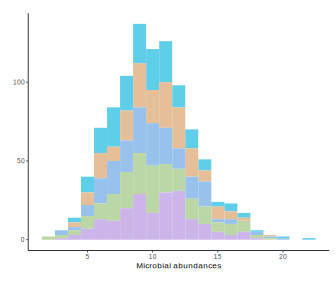
\includegraphics{report_files/mediabag/../figures/00-conceptual_figures/abundances.pdf}

}

}

\subcaption{\label{fig-conceptual-1}}
\end{minipage}%
%
\begin{minipage}[t]{0.50\linewidth}

{\centering 

\raisebox{-\height}{

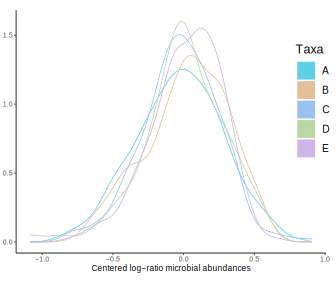
\includegraphics{report_files/mediabag/../figures/00-conceptual_figures/clr.pdf}

}

}

\subcaption{\label{fig-conceptual-2}}
\end{minipage}%
\newline
\begin{minipage}[t]{0.50\linewidth}

{\centering 

\raisebox{-\height}{


\includegraphics{report_files/mediabag/../figures/00-conceptual_figures/precision_mat.pdf}

}

}

\subcaption{\label{fig-conceptual-3}}
\end{minipage}%
%
\begin{minipage}[t]{0.50\linewidth}

{\centering 

\raisebox{-\height}{

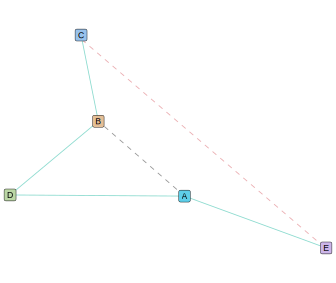
\includegraphics{report_files/mediabag/../figures/00-conceptual_figures/graph.pdf}

}

}

\subcaption{\label{fig-conceptual-4}}
\end{minipage}%

\caption{\label{fig-conceptual}\textbf{Inferring a microbial network
involves transforming the data and determining the graph structure from
a sparse precision matrix estimate.} The most popular method for
estimating a sparse precision matrix is the graphical lasso estimator.
(a) Abundances of five different taxonomic units across 200 samples. (b)
Centered log-ratio transformed abundances to address compositionality
and the assumption of normality. (c) Graphical lasso estimation of
precision matrix (\(\lambda = 0.26\)). (d) Graph structure that
corresponds to the zero-pattern of \(\hat \Omega(\lambda = 0.26)\).
False positive edges are shown in light red, and false negatives in
gray.}

\end{figure}

\hypertarget{gaussian-graphical-models}{%
\subsection{Gaussian graphical models}\label{gaussian-graphical-models}}

The following is a brief conceptualization of Gaussian graphical models
we adapted from Uhler (2017). Let \(G = (V, E)\) be an undirected graph
with nodes \(V=\{1, \dots, p\}\) and edges
\(E \subset \{(i, j) \in V\times V : i<j\}\). In our application
context, \(V\) is a set of microbial taxonomic units, although it can be
extended to include environmental factors. We define the edges of the
graph such that the absence of edge \((i, j)\) implies conditional
independence between the abundances of taxonomic units \(i\) and \(j\)
given all other variables.

We can infer the desired graph \(G\) from data by first estimating the
inverse of the covariance matrix, known as the precision matrix
\(\Omega:= \Sigma^{-1}\). The precision matrix is useful because, for
every matrix element, it is true that \(\Omega_{ij}=0\) if and only if
\(i\) and \(j\) are conditionally independent given the remaining
dimensions. We can then unambiguously determine the graph structure from
the pattern of zero entries in the precision matrix (see
Figure~\ref{fig-conceptual-3} and Figure~\ref{fig-conceptual-4}).
Formally, we say that a random variable \(X \in \mathbb R_p\) follows
\(G = (V, E)\) if it is distributed as
\(\mathcal N_p(0, \Omega ^{-1})\), where \(\Omega\) is a positive
definite matrix of dimensions \(p\times p\) such that
\(\Omega_{ij} = 0\) implies \((i, j) \notin E\). We require that
\(\Omega\) is a positive definite matrix so it is invertible, a well
known fact from linear algebra.

Research on inferring microbial networks using graphical models has
focused exclusively on estimating sparse Gaussian graphical models. The
most popular approach to induce sparsity is imposing a \(L_1\) penalty
on the precision matrix. This approach succeeded in the likelihood
framework under the name of graphical lasso (Friedman, Hastie, and
Tibshirani 2008).

\hypertarget{data-transformation}{%
\subsection{Data transformation}\label{data-transformation}}

Unfortunately, microbial abundance data is not normal (see
Figure~\ref{fig-conceptual-1}). In the literature, some methods overcome
this issue by applying a transformation to the original discrete counts.
Even worse, microbial abundance data are highly compositional because of
the unequal depth and sampling. To compare abundances between samples
the observed counts, \(\hat W\in \mathbb N_{n \times p}\), can be
normalized by the total sum of counts per sample.

However, this normalization imposes a sum-to-one constraint, making the
relative abundances \(X \in \mathbb R^+_{n\times p}\) of the different
taxonomic units no longer independent. Kurtz et al. (2015) proposed the
application of the centered log-ratio transformation (see
Equation~\ref{eq-clr}) to the relative abundances, and estimated the
Gaussian graphical model from the transformed data
\(Z \in \mathbb R_{n\times p}\) (see Figure~\ref{fig-conceptual-2}).
This is the most widely used transformation.

\begin{equation}\protect\hypertarget{eq-clr}{}{
Z_{ij} = \log \left (\frac{X_{ij}}{\left [ \prod_{m=1}^pX_{im}\right]^{\frac 1 p}}\right )
}\label{eq-clr}\end{equation}

We denote the per-sample total count sum as
\(m_i = \sum_{m=1}^p W_{i,m}\). The intuition behind the centered
log-ratio transformation is that because
\(\log{\frac {W_{i*}}{W_{j*}}} = \log{\frac {W_{i*}/m_*}{W_{j*}/m_*}} = \log{\frac {X_{i*}}{X_{j*}}}\),
the statistical inference performed with the log ratios of relative
abundances is equivalent to that performed with the log ratio of
unobserved absolute abundances (Kurtz et al. 2015).

SpiecEASI\footnote{SpiecEASI stands for \textbf{SP}arse
  \textbf{I}nvers\textbf{E C}ovariance \textbf{E}stimation for
  ecological \textbf{AS}sociation \textbf{I}nference} uses the
centered-log ratio approach (Kurtz et al. 2015), and so we have done.
However, this transformation is not exempt from criticism. Because of
the numerical problems with the geometric mean of the samples in
Equation~\ref{eq-clr}, SpiecEASI uses pseudo-counts instead of the
original values. When data are zero-inflated, the transformed data
exhibit a peak corresponding to the spike at zero, which violates the
normality assumption and might lead to spurious associations (Ha et al.
2020).

\hypertarget{inferring-an-sparse-graph}{%
\subsection{Inferring an sparse graph}\label{inferring-an-sparse-graph}}

\hypertarget{likelihood-framework}{%
\subsubsection{Likelihood framework}\label{likelihood-framework}}

In the likelihood framework, the sparse Gaussian graphical model is
usually formulated according to Friedman, Hastie, and Tibshirani (2008).

\begin{equation}\protect\hypertarget{eq-glasso}{}{
\begin{aligned}
\mathcal L(\Omega) = \log |\Omega| - \text{trace}(\hat \Sigma \Omega)\\
\hat \Omega(\lambda) = \arg \min_{\Omega\in M^+} (-L(\Omega) + \lambda ||\Omega||_1)
\end{aligned}
}\label{eq-glasso}\end{equation}

where \(M^+\) is the set of positive definite matrices, \(\hat \Sigma\)
is the empirical covariance matrix, and \(||\Omega||_1\) is the \(L_1\)
norm (the sum of all the absolute values of the matrix).
\(\mathcal L(\Omega)\) is the log-likelihood of the data after
maximizing the mean vector \(\mu\) and ignoring constants. \(\lambda\)
is a positive regularization parameter that controls the sparsity of the
estimated precision matrix, \(\hat \Omega(\lambda)\), and consequently,
of graph \(G(\lambda)\).

Friedman, Hastie, and Tibshirani (2008) proposed an algorithm that
efficiently solves the optimization problem shown in
Equation~\ref{eq-glasso}. Previously, Meinshausen and Bühlmann (2006)
suggested that it is sufficient to estimate the pattern of zero
elements, rather than the whole matrix to determine the graph. This
pattern can be inferred by fitting \(p\) lasso regressions and using
each variable as the response variable. Let us denote as
\(\hat\beta_a^b\) the \(a\)-coefficient of the lasso regression with the
\(b\) variable as the response for a given value of \(\lambda\). Their
method constrains the estimated graph by excluding all edges \((i, j)\)
where either \(\hat\beta_i^j = 0\) or \(\hat\beta_j^i = 0\).

The sparsity of the true graph, thus, of the true unknown precision
matrix, is unknown. The challenge faced by likelihood-based methods is
the selection of an appropriate value of \(\lambda\). Different criteria
may be used, such as selecting \(\lambda\) so it optimizes the Akaike
information criterion, the Bayesian information criterion, or the
largest within one standard error of the optimal negative likelihood
when performing cross-fold validation (or any equivalent rule of thumb)
(Liu, Roeder, and Wasserman 2010). However, since the publication of the
SpiecEASI method (Kurtz et al. 2015), nearly all microbial co-occurrence
network inferences have used the StARS\footnote{StARS stands for
  Stability Approach to Regularization Selection.} selection method
(Liu, Roeder, and Wasserman 2010).

The StARS method is a general procedure that can be applied to any
graph-inference method. However, the authors built it on top of the
Meinshausen and Bühlmann method. Despite its simplicity, it provides
better results in terms of speed, recall and precision than the
alternatives (Kurtz et al. 2015). The core idea of StARS is to draw many
random overlapping subsamples (without replacement) and apply the
Meinshausen and Bühlmann method to each subsample with decreasing values
of \(\lambda\) until there is a small but acceptable amount of
variability.

They defined the variability in terms of the average total instability
of the edges. Specifically, for any chosen \(\lambda\), they estimate
\(m\) graphs, one for each \(m\) subsample. They calculated the
instability of a particular edge \((i, j)\) as the fraction of every
possible pair of \(m\) graphs that disagree in the presence or absence
of an \((i, j)\) edge. Liu, Roeder, and Wasserman (2010) stated that
they could estimate a graph containing the true graph with high
probability by selecting the largest value of \(\lambda\) (the sparsest
graph) for which the average total instability is equal to or more than
\(\beta\). They claimed that this cut-off point \(\beta\) is an
interpretable quantity (so they did not simply replace the problem of
choosing \(\lambda\) to choose \(\beta\)) and that a reasonable default
value is \(\beta = 0.05\).

\hypertarget{bayesian-framework}{%
\subsubsection{Bayesian framework}\label{bayesian-framework}}

Different versions of the graphical lasso estimator have been proposed
in the Bayesian framework (Wang 2012; Piironen and Vehtari 2017; Richard
Li, McCormick, and Clark 2019; Li, Craig, and Bhadra 2019). However, its
application to microbial co-occurrence network inference is not entirely
satisfactory. Because the lasso prior places no probability of any value
of the precision matrix being exactly zero, \(\Omega_{ij}=0\), there is
no probability of the event \(\Omega_{ij}=0\) in the posterior either.
This means that we require a \emph{post hoc} heuristic to include or
exclude an edge from the inferred sparse graph (which is our desired
estimand, not the precision matrix). For example, that all off-diagonal
elements are set to zero if the 95\% credibility interval contains a
zero value (Jongerling, Epskamp, and Williams 2023).

The alternative is to use a family of priors called G-Wishart, which is
a discrete and continuous mixture prior distribution. If so, we estimate
the joint posterior distribution of the precision matrix and graph, as
shown in Equation~\ref{eq-join-post}.

\begin{equation}\protect\hypertarget{eq-join-post}{}{
P(G, \Omega|Z) \propto P(Z|G, \Omega) P(\Omega|G)P(G)
}\label{eq-join-post}\end{equation}

\(P(Z|G, \Omega)\) corresponds to the likelihood function of a
multivariate normal distribution, as in the frequentist graphical lasso.
The G-Wishart distribution is a convenient prior choice for the
precision matrix, \(P(\Omega|G)\), because it is conjugated with this
likelihood (Roverato 2002). The G-Wishart distribution of a given graph,
\(W_G(b, D)\), depends on the number of degrees of freedom \(b>2\) and
the matrix \(D\in M^+\) which is usually set to be the identity matrix.
Note that, in Equation~\ref{eq-probomega}, we ensure \(\Omega\) is a
valid precision matrix by multiplying the probability by the indicator
variable \(\mathbb 1_{\Omega\in M ^+}\) (i.e., setting the probability
of any nonpositive definite matrix to zero).

\begin{equation}\protect\hypertarget{eq-probomega}{}{
P(\Omega|G) \propto |\Omega|^{(b-2)/2} \exp\left \{ -\frac 1 2 \text{trace}(D\Omega)  \right\} \mathbb 1_{\Omega\in M ^+}
}\label{eq-probomega}\end{equation}

Many priors have been proposed for the graph structure, \(P(G)\) (Jones
et al. 2005; Carvalho and Scott 2009; A. Mohammadi and Wit 2015). A
popular choice depends on a \(\theta \in (0, 1)\) parameter that
expresses our prior belief in the sparsity of the graph (see
Equation~\ref{eq-probg}). The larger the graph size, i.e.~the number of
edges, denoted by \(|E|\), the less likely the graph is. Note that, if
\(\theta = 0.5\), the distribution corresponds to a uniform distribution
over the entire graph space.

\begin{equation}\protect\hypertarget{eq-probg}{}{
P(G) \propto \left ( \frac{\theta}{1-\theta}\right) ^{|E|}
}\label{eq-probg}\end{equation}

To explore the graph space and estimate the model parameters
simultaneously, we need a particular type of algorithm, the so-called
trans dimensional Markov Chain Monte Carlo (A. Mohammadi and Wit 2015).
Unfortunately, the graph space is exponentially large\footnote{Specifically,
  \(2^{p(p-1)/2}\) graphs exist.} and convergence is complex. A.
Mohammadi and Wit (2015) proposed a birth-death MCMC, which works well
in practice. Every edge is added or removed according to two independent
Poisson birth and death processes. The algorithm is formulated such that
the posterior distribution of a graph is proportional to how much time
the sampling algorithm remained in a particular graph after a certain
amount of iterations.

In contrast to the likelihood method, the estimate we obtain is the full
posterior distribution \(P(G, \Omega|Z)\). A graph point estimate is
usually estimated by Bayesian model averaging. First, the average edge
inclusion probability of every possible edge is computed as the fraction
of times that edge was found in the sampled graphs. Then, a graph is
constructed with all the edges whose probability is greater than a
specified threshold.

\hypertarget{results}{%
\section{Results}\label{results}}

\hypertarget{simulation-of-synthetic-datasets}{%
\subsection{Simulation of synthetic
datasets}\label{simulation-of-synthetic-datasets}}

We simulated data for 53 graphs from different topology and graph sizes
(see Figure~\ref{fig-networks}). First, we simulated a graph and normal
multivariate data such that their precision matrix was compatible with
it. We then simulated microbial abundances that correlated with the
normal multivariate distribution. The abundance of each taxonomic unit
was drawn from a negative binomial distribution and unequal depths
between the samples. For more details, see the Methods section.

\begin{figure}

\begin{minipage}[t]{0.50\linewidth}

{\centering 

\raisebox{-\height}{

\includegraphics{../figures/11-network_plots/random_500.pdf}

}

}

\subcaption{\label{fig-random1}Random network (Graph size = 193)}
\end{minipage}%
%
\begin{minipage}[t]{0.50\linewidth}

{\centering 

\raisebox{-\height}{

\includegraphics{../figures/11-network_plots/random_100.pdf}

}

}

\subcaption{\label{fig-random2}Random network (Graph size = 120)}
\end{minipage}%
\newline
\begin{minipage}[t]{0.50\linewidth}

{\centering 

\raisebox{-\height}{

\includegraphics{../figures/11-network_plots/cluster_100.pdf}

}

}

\subcaption{\label{fig-cluster}Cluster network (Graph size = 184)}
\end{minipage}%
%
\begin{minipage}[t]{0.50\linewidth}

{\centering 

\raisebox{-\height}{

\includegraphics{../figures/11-network_plots/hub_100.pdf}

}

}

\subcaption{\label{fig-hub}Hub network (Graph size = 294)}
\end{minipage}%

\caption{\label{fig-networks}We analyzed three representative network
topologies: random, hub, and cluster. The subfigures show four randomly
simulated networks with 100 nodes (taxonomic units) and different
numbers of edges (graph size).}

\end{figure}

\hypertarget{recovery-of-microbial-networks}{%
\subsection{Recovery of microbial
networks}\label{recovery-of-microbial-networks}}

\begin{figure}

\begin{minipage}[t]{\linewidth}

{\centering 

\raisebox{-\height}{

\includegraphics{../figures/01-precision-recall/f1-normal.pdf}

}

}

\subcaption{\label{fig-prec_recall_normal}Multivariate normal data}
\end{minipage}%
\newline
\begin{minipage}[t]{\linewidth}

{\centering 

\raisebox{-\height}{

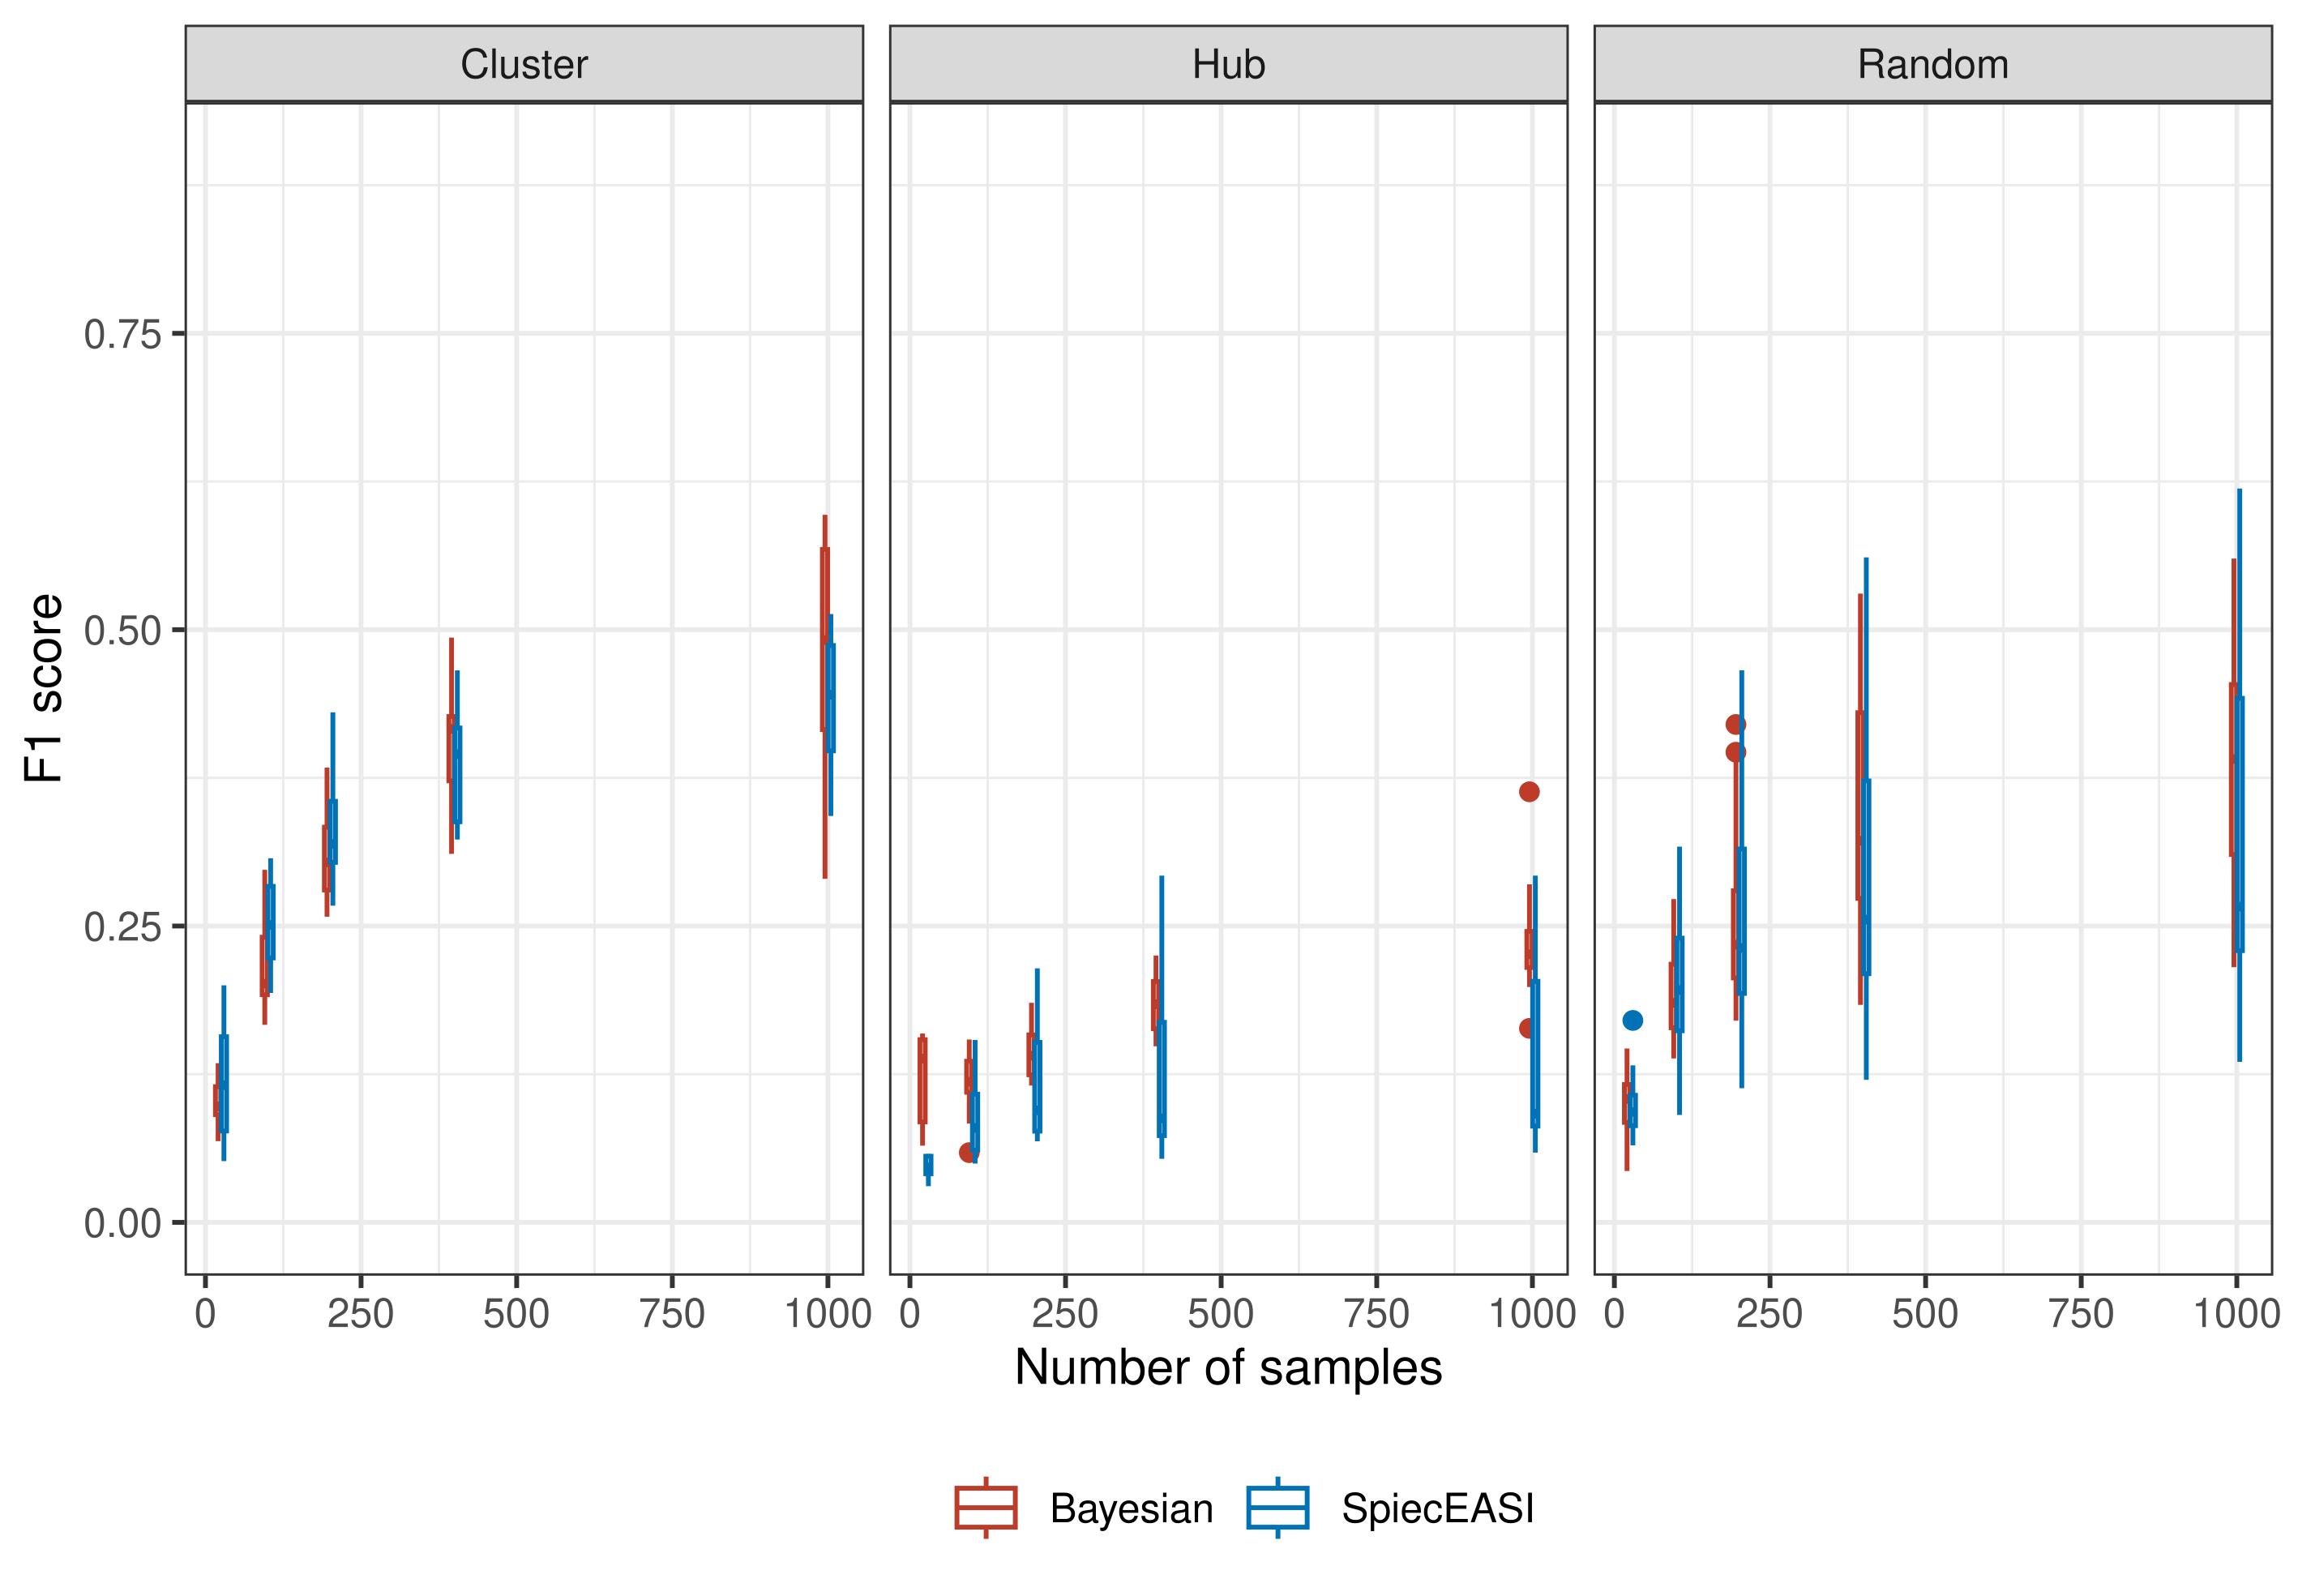
\includegraphics{../figures/01-precision-recall/f1-counts.pdf}

}

}

\subcaption{\label{fig-prec_recall_counts}CLR -transformed microbial
counts}
\end{minipage}%

\caption{\label{fig-prec_recall}Recovery depends on sample size,
underlying network topology, and data type. We show the F1 score across
different data types, sample sizes, and methods. All the networks
contained 100 nodes (taxonomic units). A total of 1590 models were
evaluated.}

\end{figure}

We evaluated the recovery of the true graph from datasets of increasing
sample size. We analyzed the 53 graphs and their respective data. In
addition to microbial counts, to which we applied the centered log-ratio
transformation, we evaluated performance when inference was performed
with the noiseless normal multivariate data. The latter would correspond
to performing the inference as if we had access to the latent random
variables.

As mentioned before, we considered two methods: SpiecEASI and its
Bayesian alternative with a G-Wishart prior based on BDgraph. More
specifically, we assessed the completeness of the optimal graph selected
by SpiecEASI when setting \(\beta=0.05\), and of the Bayesian method
when predicting the graphs of all the edges whose posterior inclusion
probability was greater than \(0.5\). Both strategies were the default
strategies in their respective R libraries.

\hypertarget{f1-score}{%
\subsubsection{F1-score}\label{f1-score}}

Figure~\ref{fig-prec_recall} shows the F1-score for different sample
sizes and datasets. The F1-score summarizes precision (number of
true-positive edges divided by the number of edges) and recall (number
of true-positive edges divided by the number of true edges). For both
the methods, the inference improved with the sample size. We observed
differences among the three topologies, with the most challenging being
the hub topology. Linking the data to microbial counts and applying the
centered log-ratio transformation afterward adversely affected recovery,
which became more weakly dependent on the sample size (see
Figure~\ref{fig-prec_recall_counts}). The inference for a sample size of
25 was poor in all the cases (F1 \textless{} 0.25).

The Bayesian method performed significantly better than SpiecEASI with
both normal-multivariate data and microbial counts (p = 6.6e-07 and p =
9.4e-09 from a paired-Welch test on the difference of F1 means).
SpiecEASI exhibited greater variability than the Bayesian method when
considering a fixed graph structure and sample size. A portion of this
variability can be attributed to the differences in the maximum
degree\footnote{The maximum degree is the number of edges of the most
  connected node in a graph, and it plays an important role in
  determining the number of samples required to recover the true graph
  (Kurtz et al. 2015)}, denoted by \(d\), across various simulated
graphs. We found the \(d\) term to be significant in a likelihood ratio
test (p =1.3e-14) for SpiecEASI but not for the Bayesian method.

\hypertarget{precision-versus-recall}{%
\subsubsection{Precision versus recall}\label{precision-versus-recall}}

\begin{figure}

{\centering 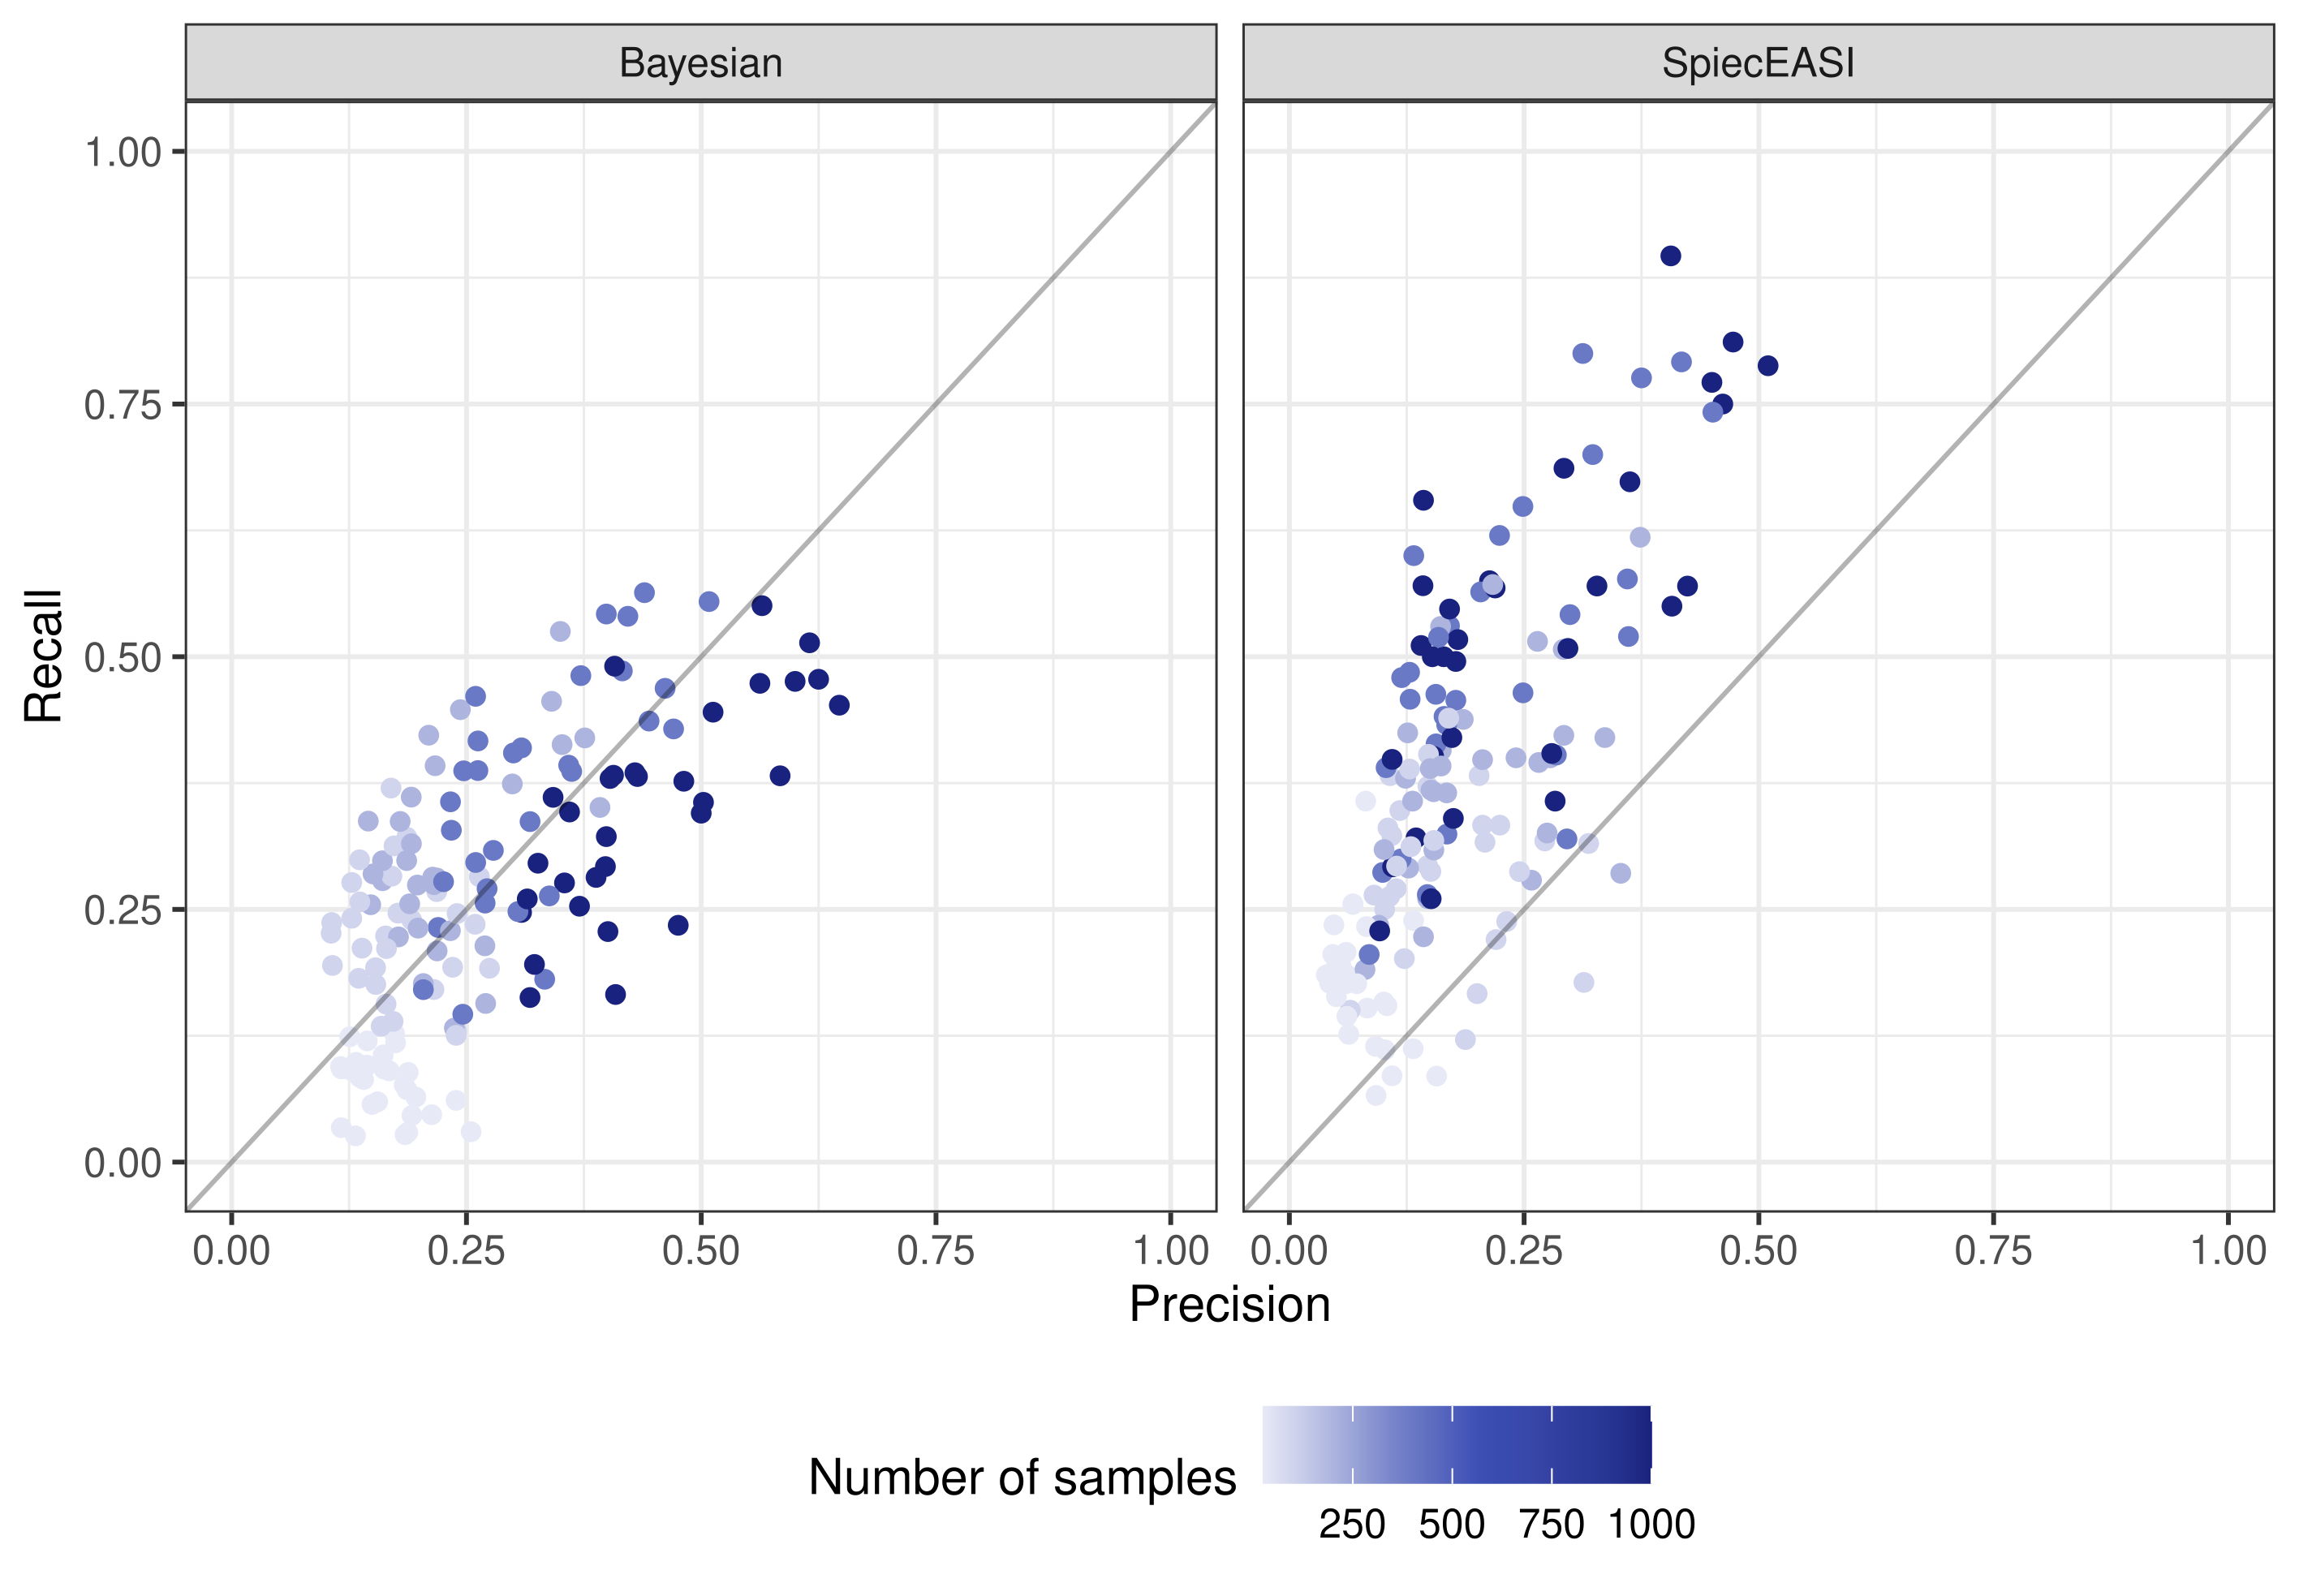
\includegraphics{../figures/01-precision-recall/prec_recall-counts.pdf}

}

\caption{\label{fig-precision_recall_counts}SpiecEASI tended to
over-select the edges. We show the recall versus the precision of the
same models as Figure~\ref{fig-prec_recall_counts} (only microbial
counts) across different sample sizes.}

\end{figure}

SpiecEASI tended to overselect edges, so we obtained more complete
graphs at the cost of more spurious edges (see
Figure~\ref{fig-precision_recall_counts}). In contrast, the Bayesian
method had a more balanced distribution of error types, which was a
consequence of the established inclusion threshold \(\alpha=0.5\). With
microbial counts, precision was rarely greater than 50\% for any of the
methods.

\hypertarget{k-top-ranked-edges}{%
\subsubsection{\texorpdfstring{\(k\) top-ranked
edges}{k top-ranked edges}}\label{k-top-ranked-edges}}

We considered the analysis of only the top-ranked edges. We assessed the
proportion of incorrect edges when only edges with the highest
confidence were considered. We compared both methods by including the
\(k\) top-ranked edges (see Figure~\ref{fig-ranked}) according to their
inclusion probability (Bayesian method) or their stability between
resamples (SpiecEASI).

The success of this strategy was highly dependent on sample size.
However, it provided better results for the SpiecEASI, especially for
small samples. Our results suggest that obtaining relatively high
precision (above 50\%) might be feasible if we restrict our analysis to
the \(k\)-top ranked edges. We discuss the difficulty of choosing \(k\)
later.

\begin{figure}

{\centering \includegraphics{../figures/09-ranked_edges/plot.pdf}

}

\caption{\label{fig-ranked}Selecting the \(k\) top-ranked edges of
SpiecEASI improved the accuracy for small sample sizes. We show
precision when predicting only the presence of the top \(k\)-ranked
edges. We ranked the edges according to the probability of inclusion
(Bayesian) and the stability between resamples (SpiecEASI). Different
lines show the tendencies across sample sizes. We included randomly
sampled points from the dataset for better visualization. We evaluated
the expected precision when selecting edges randomly (gray baseline).}

\end{figure}

\hypertarget{predicting-network-properties}{%
\subsection{Predicting network
properties}\label{predicting-network-properties}}

We analyzed the error of three representative metrics across increasing
sample sample sizes: modularity, hub score, and distances between
taxonomic units. The Bayesian method performed better on the three
metrics and it was more robust to variations in true networks than the
SpiecEASI method. This result was consistent across topologies, graph
sizes, and dataset types (normal multivariate or microbial counts).

\begin{figure}

\begin{minipage}[t]{\linewidth}

{\centering 

\raisebox{-\height}{

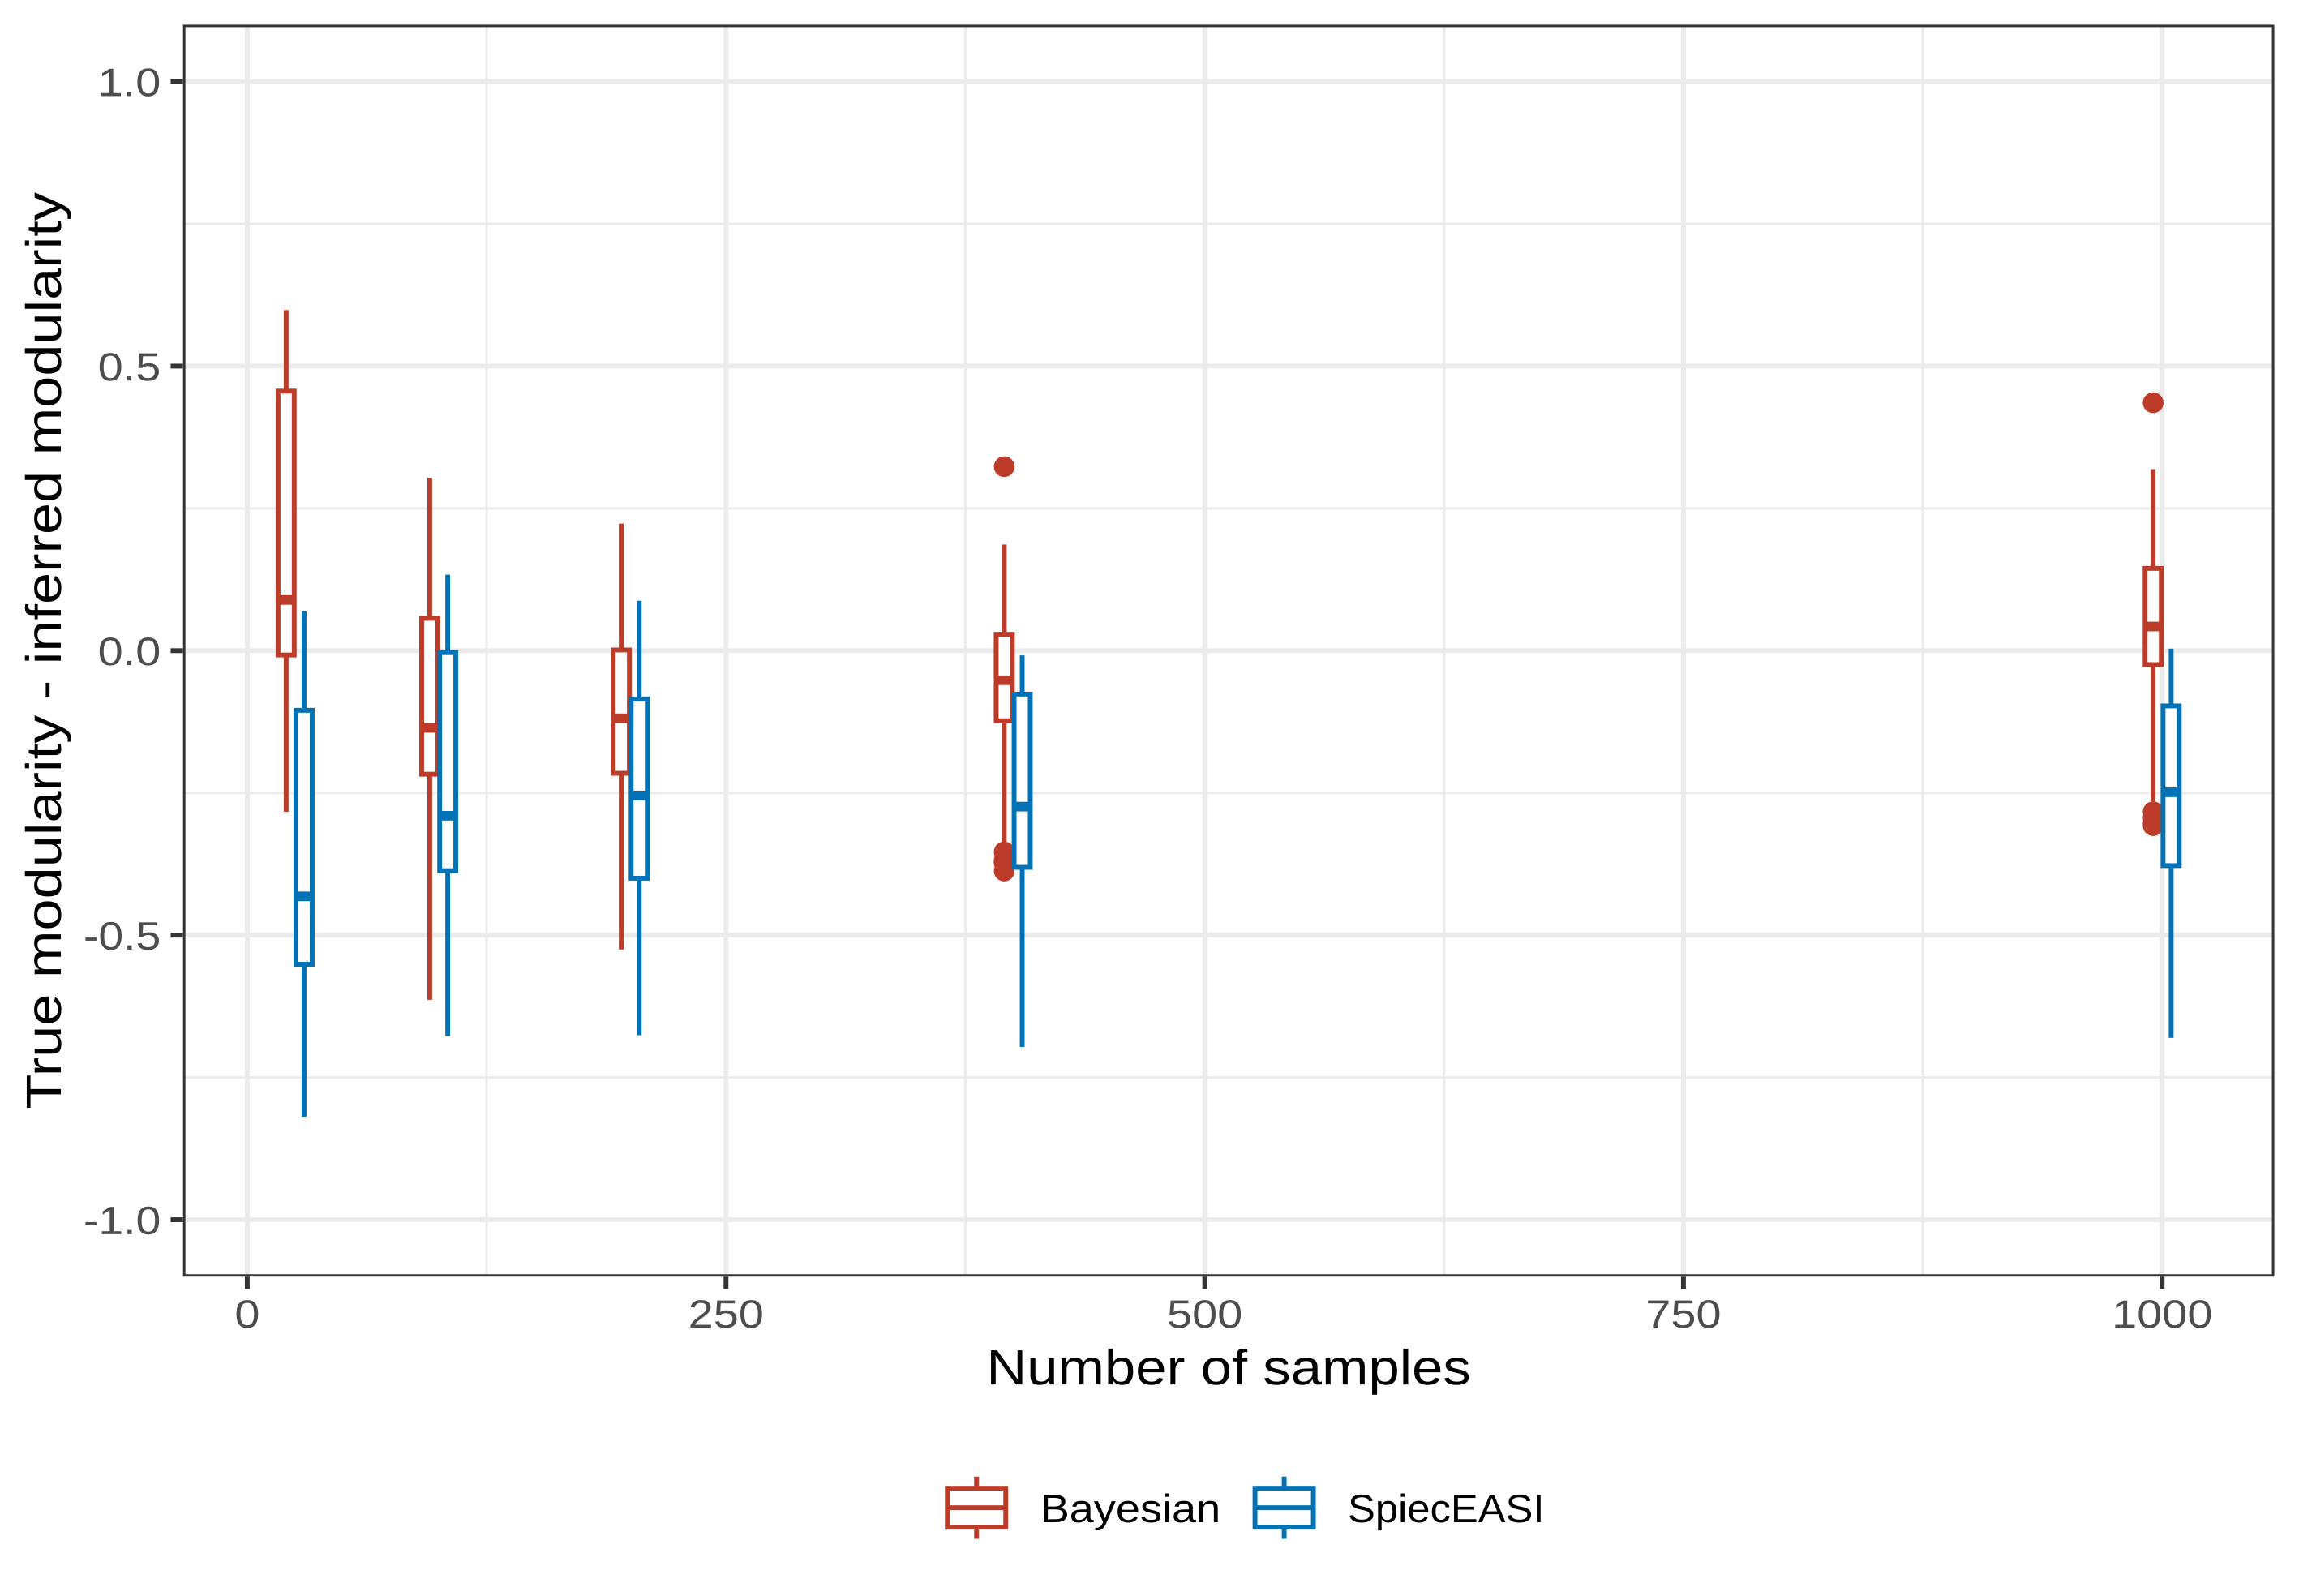
\includegraphics{../figures/07-regression_combined/modularity_boxplot.pdf}

}

}

\subcaption{\label{fig-mod}}
\end{minipage}%
\newline
\begin{minipage}[t]{\linewidth}

{\centering 

\raisebox{-\height}{

\includegraphics{../figures/07-regression_combined/hub_score.pdf}

}

}

\subcaption{\label{fig-hubscore}}
\end{minipage}%

\caption{\label{fig-regression}The predicted network properties may be
unreliable, especially for low sample sizes. We show the results for the
same models as Figure~\ref{fig-prec_recall_counts} (microbial counts
only). (a) Differences between the true and predicted modularities. (b)
Mean square error (MSE) of each node's true and predicted hub scores.}

\end{figure}

Regarding modularity, the error was considerably high, especially at low
sample size, for both methods (see Figure~\ref{fig-mod}). SpiecEASI
systematically overestimated modularity. The mean square error (MSE) of
the hub scores was relatively low, below 30\% even when \(n<p\) (see
Figure~\ref{fig-hubscore}). The distances between nodes were the least
reliable metrics. Unlike the modularity and hub score, which did not
improve substantially, the sample size affected the correlation between
the true and inferred distances greatly. For low sample size, \(n<p\),
the Spearman correlation was systematically poor (close to zero).

\hypertarget{module-identification}{%
\subsection{Module identification}\label{module-identification}}

We evaluated the reliability of modules of taxonomic units co-occurring
together. We clustered the networks after excluding edges that
corresponded to negative correlations using the Walktrap algorithm (Pons
and Latapy 2005). We compared the true and inferred clusters using the
adjusted mutual information (AMI). The AMI metric compares the
similarity between two partitions of potentially different sizes, and
takes a value of one if both partitions are identical and zero when the
overlap equals the expected by chance alone (Vinh, Epps, and Bailey
2009).

The obtained clusters were surprisingly reliable, and SpiecEASI (not
using the Meinshausen and Bühlmann method, but estimating the whole
precision matrix) was consistently better than the Bayesian alternative
(see Figure~\ref{fig-ami}). Even for a middle sample size, meaningful
clusters can be obtained.

\begin{figure}

{\centering 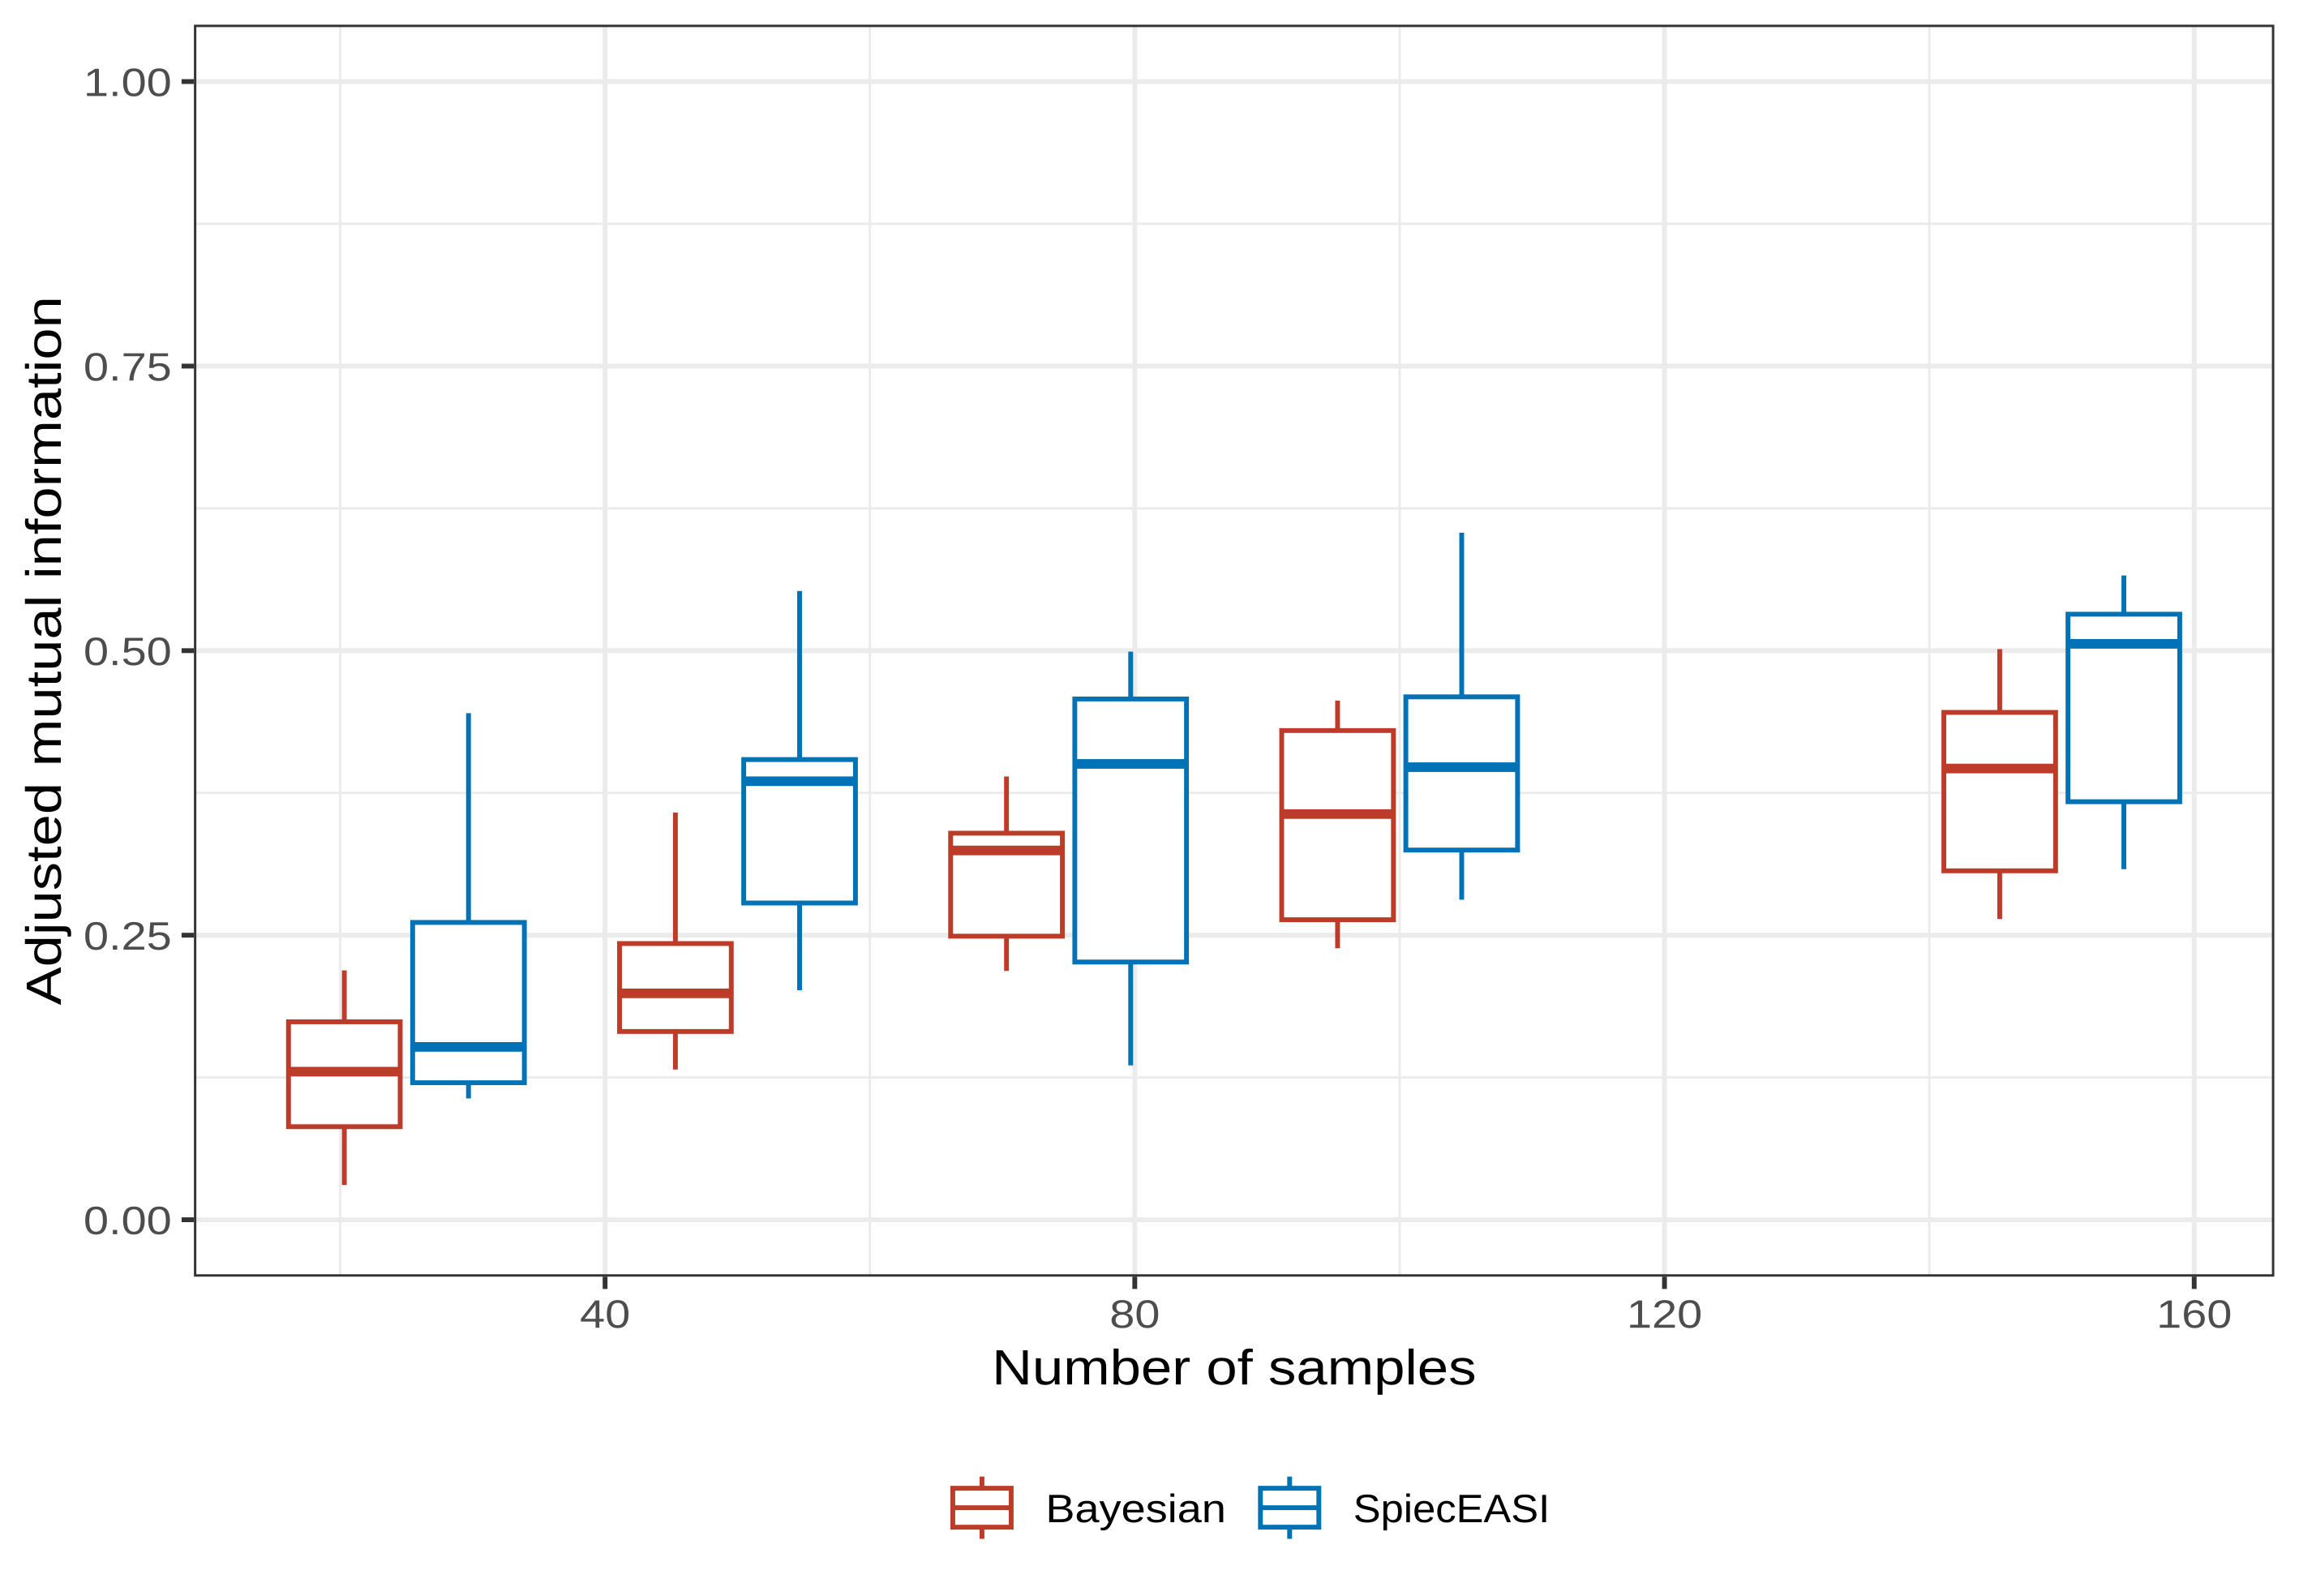
\includegraphics{../figures/10-cluster_niche_preference/cluster_ami.pdf}

}

\caption{\label{fig-ami}SpiecEASI provides more reliable cluster
partitions. We show the adjusted mutual information between the true and
predicted clusters for five networks across different sample sizes.
Clusters were obtained only by considering positive correlations between
taxonomic units.}

\end{figure}

\hypertarget{confidence-and-credibility-intervals}{%
\subsection{Confidence and credibility
intervals}\label{confidence-and-credibility-intervals}}

Finally, we computed bootstrapping confidence intervals for SpiecEASI
and credibility intervals for the Bayesian method. We did it for all
previous metrics except for module identification. To our knowledge, the
BDgraph implementation does not provide posterior samples of the
precision matrix, so we did not compute any credibility intervals
involving the sign of the edges.

\begin{figure}

\begin{minipage}[t]{\linewidth}

{\centering 

\raisebox{-\height}{

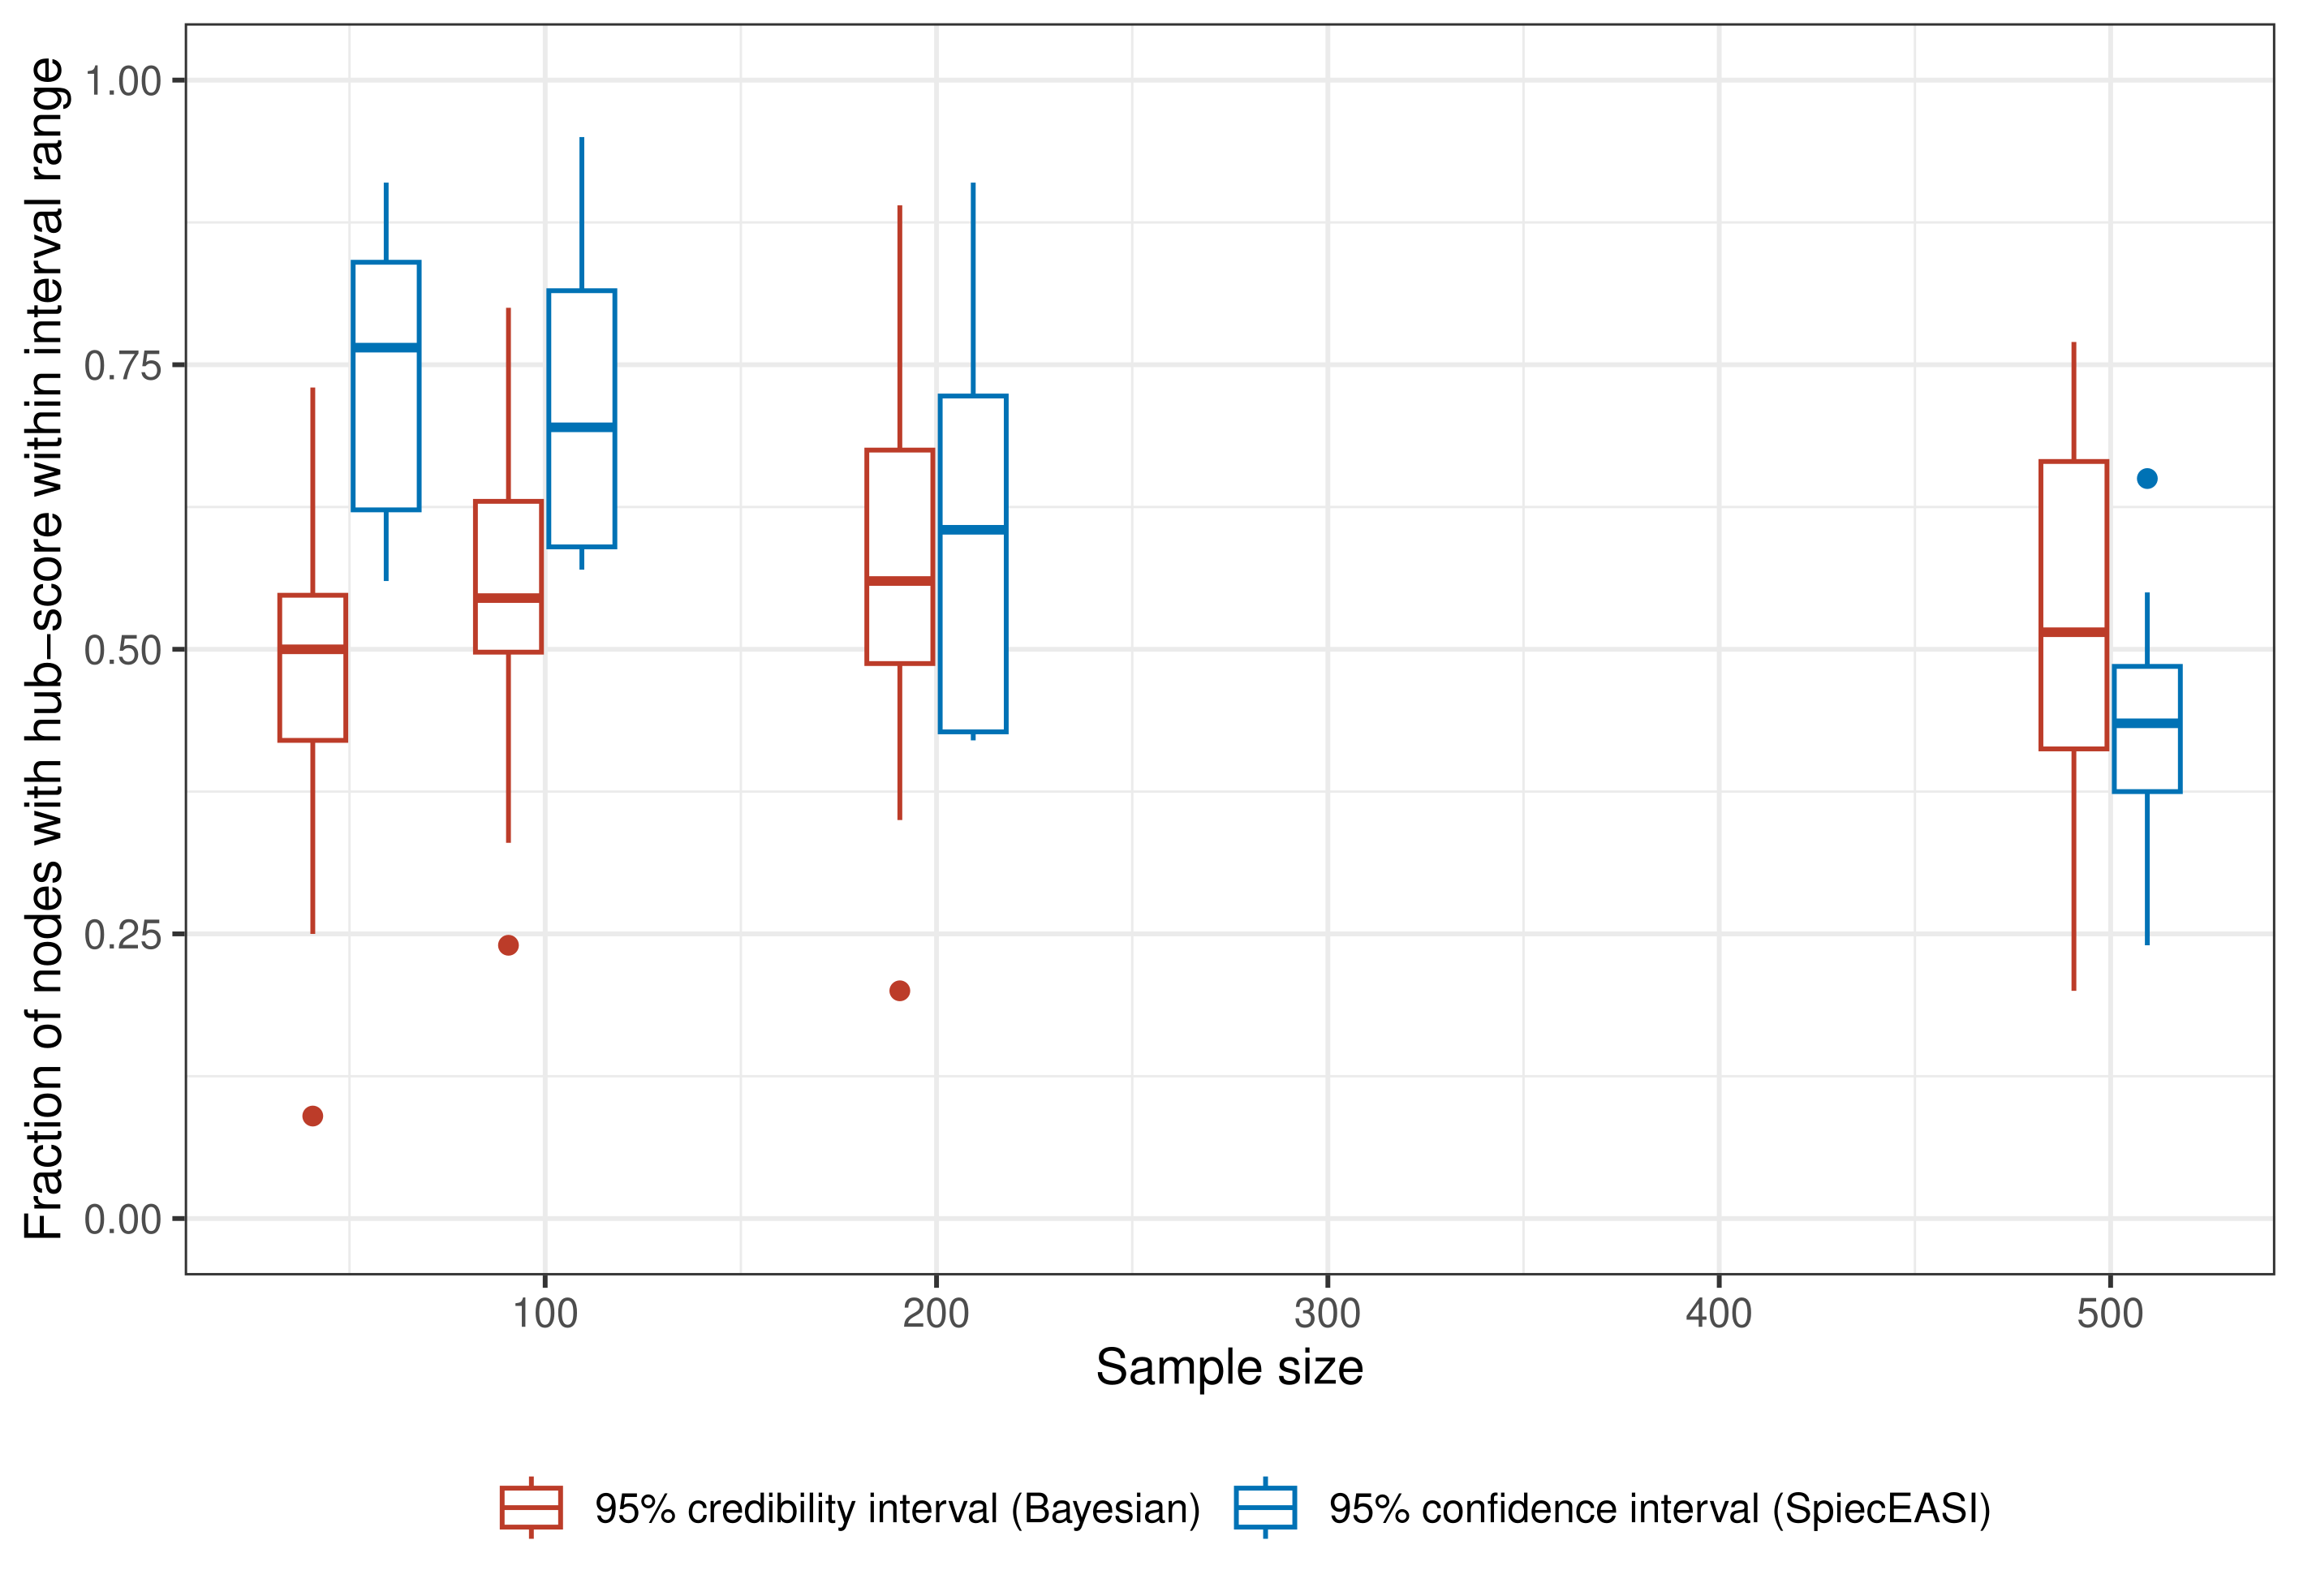
\includegraphics{../figures/03-credibility-confidence/hub_nodewise_contain.pdf}

}

}

\subcaption{\label{fig-nodewise_contain}Fraction of nodes with hub-score
within the 95\% credibility or confidence interval}
\end{minipage}%
\newline
\begin{minipage}[t]{\linewidth}

{\centering 

\raisebox{-\height}{

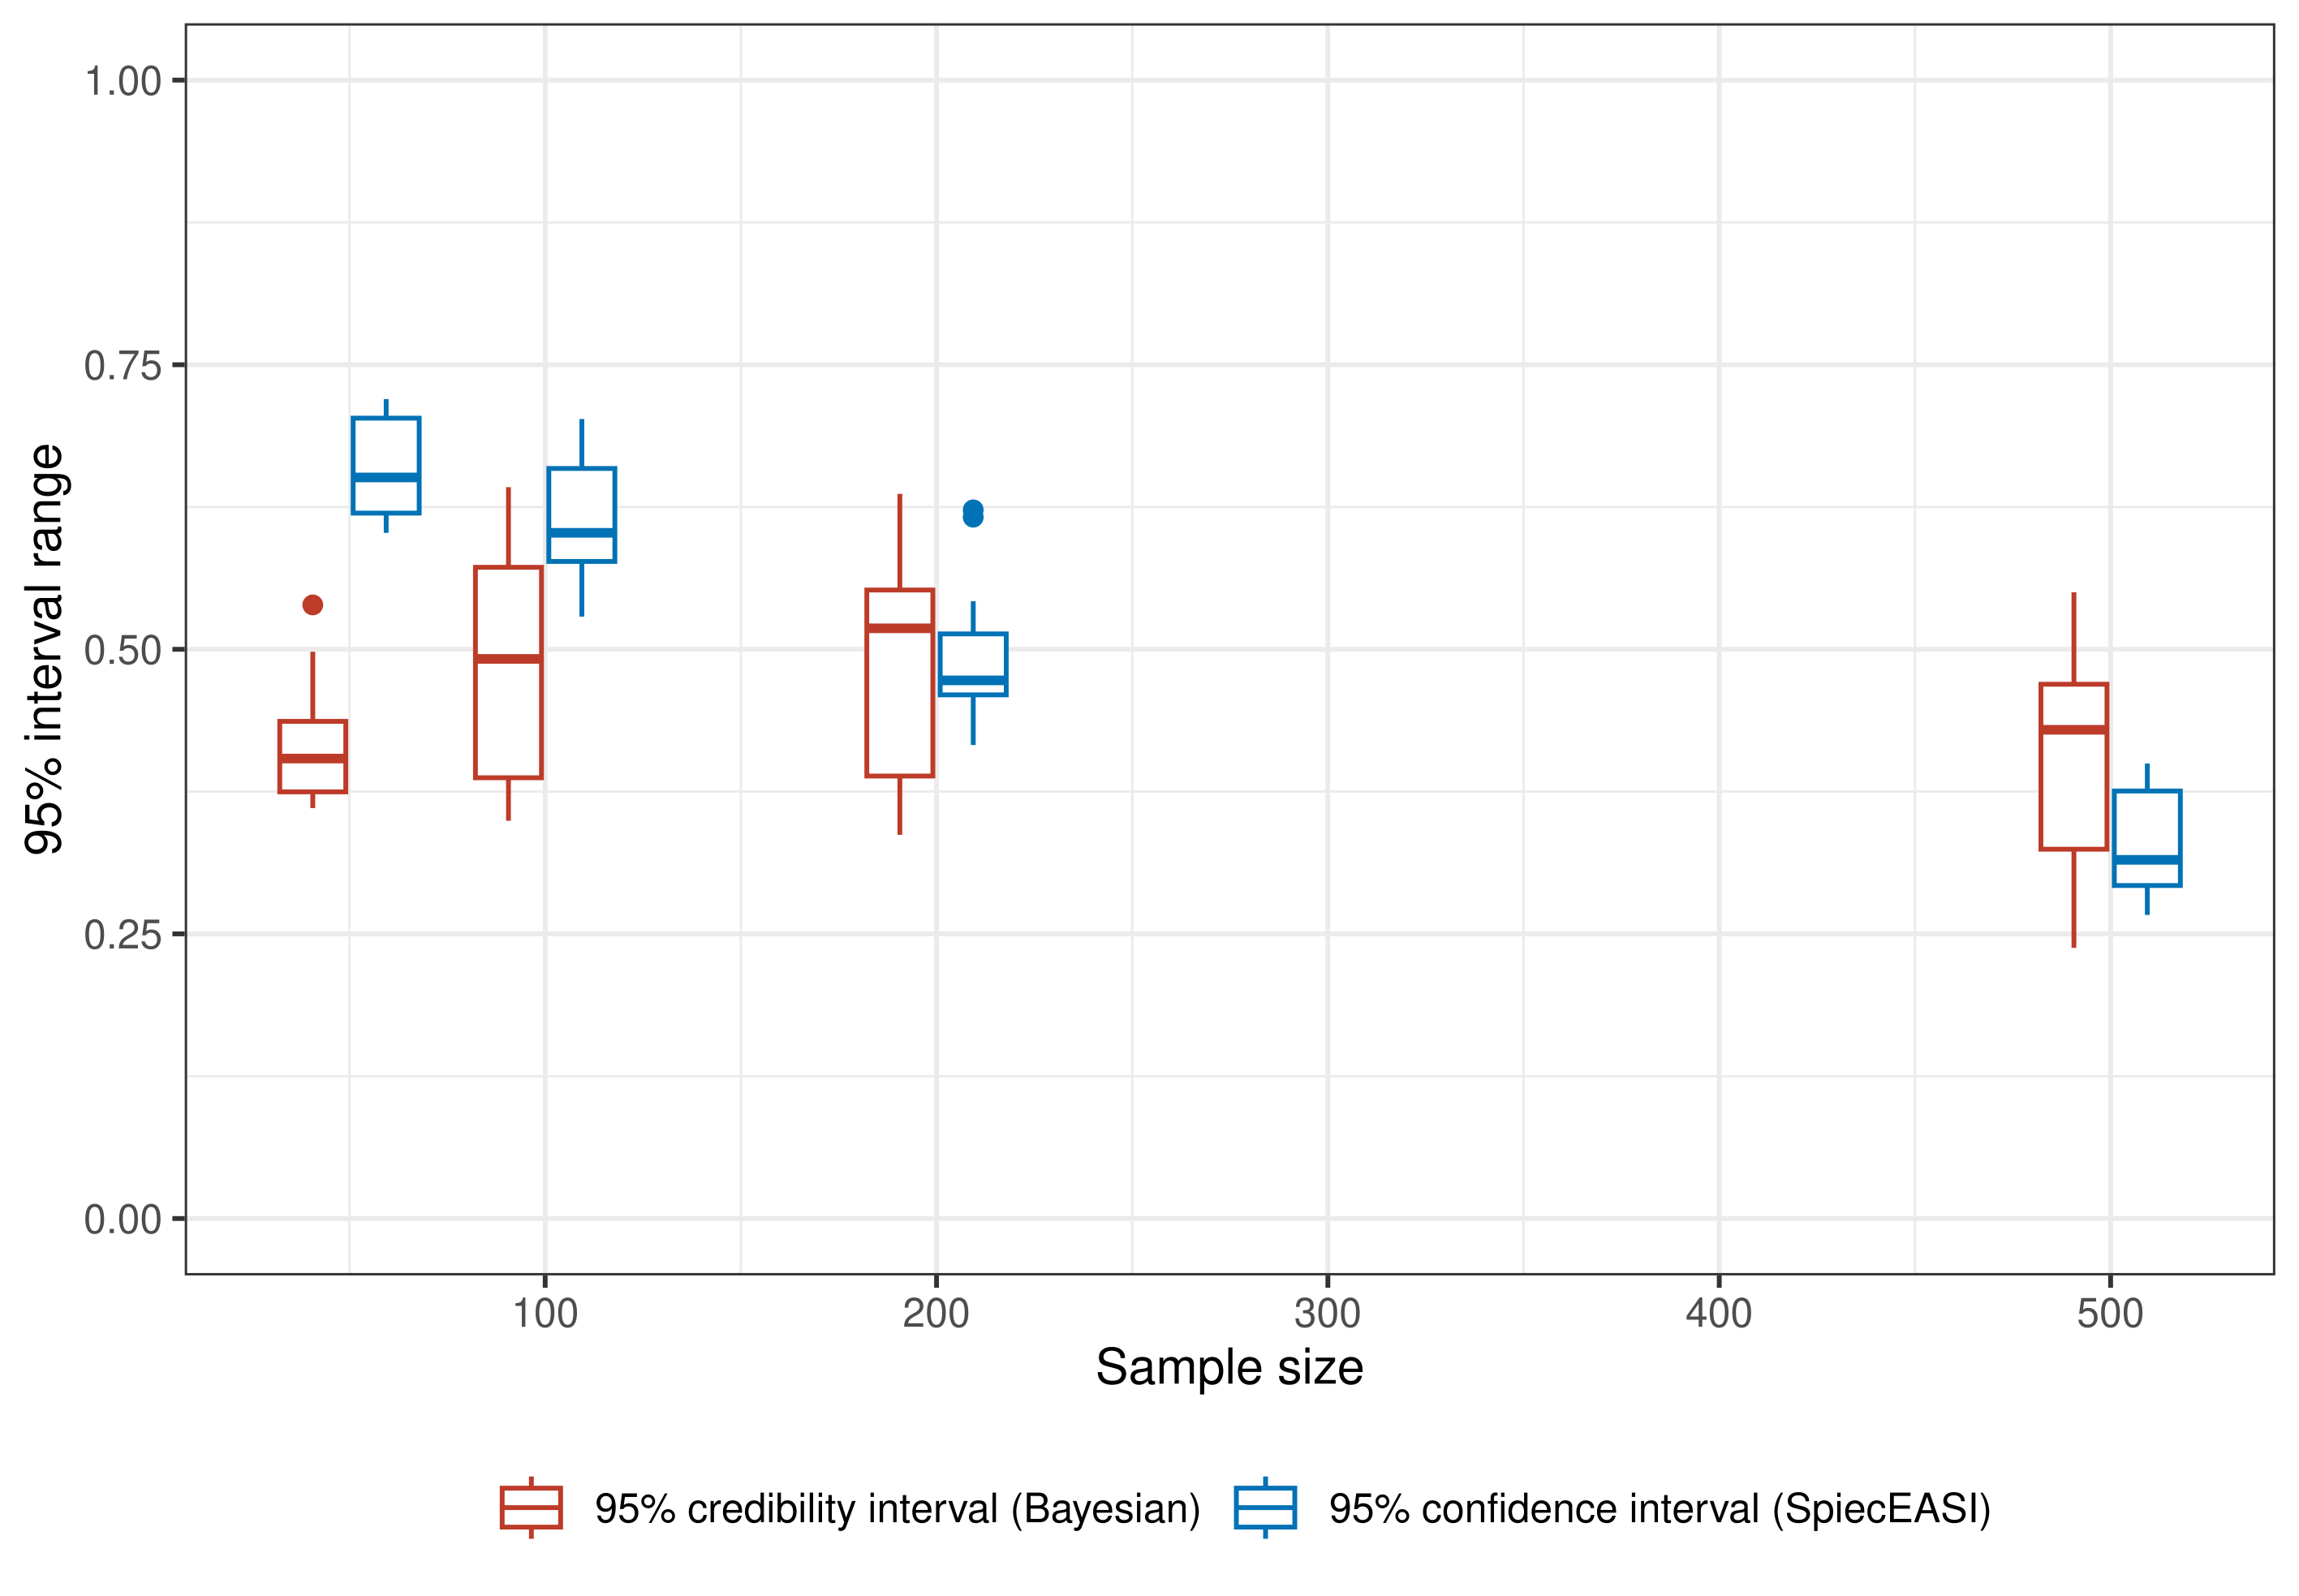
\includegraphics{../figures/03-credibility-confidence/hub_nodewise_size.pdf}

}

}

\subcaption{\label{fig-nodewise_size}95\% credibility or confidence
interval range}
\end{minipage}%

\caption{\label{fig-intervals}The use of credibility or confidence
intervals is unlikely to increase statistical robustness. We show the
results for ten random networks estimated from microbial counts with low
sample sizes. (a) Fraction of nodes whose true values are within the
95\% credibility or 95\% confidence interval. (b) Range of each interval
(i.e., \(Q_{0.975} - Q_{0.025}\)).}

\end{figure}

We show the results only of the hub score estimated from microbial, as
it is the one we analyzed in more detail (see
Figure~\ref{fig-nodewise_size}). We chose this metric because it is the
most well-known. Similar results were obtained for the other measures
when estimating microbial counts. The 95\% confidence intervals were
wide, as their range was between 25\% and 75\% of the entire range of
possible values (from zero to one). The fraction of nodes whose
credibility or confidence interval contains their true hub score
oscillates within the same range.

There is a negative relationship between the number of samples and the
bootstrap confidence interval range for SpiecEASI. The fraction of nodes
with their true hub score within their 95\% confidence interval
decreases similarly when the sample size is increased (i.e., increasing
the sample size narrows the confidence interval but not around the true
value).

The Bayesian model showed a very narrow confidence interval for a small
sample size (as it tends to predict sparse networks). For larger sample
sizes, a very weak negative correlation was observed. We saw no big
improvements for the Bayesian method when increasing the sample size, as
the fraction of nodes' hub scores within their 95\% credibility interval
oscillated around 25\% and 75\%.

\hypertarget{methods}{%
\section{Methods}\label{methods}}

All the scripts used in this project can be found in
\href{https://github.com/currocam/microbial-network-inference}{github.com/currocam/microbial-network-inference}.
All statistical analysis was done in R (R Core Team 2021).

\hypertarget{simulation-of-synthetic-datasets-1}{%
\subsection{Simulation of synthetic
datasets}\label{simulation-of-synthetic-datasets-1}}

Random networks were simulated by assigning a Bernoulli random variable,
where \(p\) was fixed for every network and drawn from a uniform
distribution between 0.01 and 0.1. The hub networks were simulated by
assigning each node to a random \(g\) group. Each group is then assigned
a center (from itself) and one edge is inserted for every node with its
center. The number of hubs \(g\) was randomly chosen as an integer from
one to ten. The cluster networks were simulated by assigning each node
to a random \(g\) group ( sampled from 1 to 10). We then assigned a
Bernoulli random variable with \(p=0.2\) between every pair of nodes
belonging to the same group.

We used BDgraph to simulate data from a negative binomial distribution
such that its correlations were consistent with the simulated graphs (R.
Mohammadi and Wit 2019). We simulated unequal depth sequencing by
multiplying by a correction factor (sampled from a uniform distribution
{[}0.75, 1.25{]}).

\hypertarget{fitting-graphical-models-with-spieceasi}{%
\subsection{Fitting graphical models with
SpiecEASI}\label{fitting-graphical-models-with-spieceasi}}

We fitted graphical models using the Pulsar implementation (Müller,
Bonneau, and Kurtz 2016), as described by Kurtz et al. (2015). A
single-threaded Julia implementation was also made and it is available
in the repository
(\href{https://github.com/currocam/microbial-network-inference/blob/main/src/StARS_MB.jl}{github.com/currocam/microbial-network-inference/blob/main/src/StARS\_MB.jl}).

\hypertarget{fitting-graphical-models-with-bdgraph}{%
\subsection{Fitting graphical models with
BDgraph}\label{fitting-graphical-models-with-bdgraph}}

We used the birth-death MCMC algorithm (R. Mohammadi and Wit 2019), with
10000 iterations, 5000 burn-in iterations and a single chain. We
assigned an uninformative prior to the graph space (all graphs are
equally plausible) but set the initial graph to be empty. The chosen
G-Wishart prior distribution has two degrees. We assessed the
convergence by tracing the graph size across the chain.

\hypertarget{recovery-of-microbial-networks-1}{%
\subsection{Recovery of microbial
networks}\label{recovery-of-microbial-networks-1}}

We assessed the recovery of both methods by comparing the adjacency
matrix of the true and inferred graph. The likelihood ratio test was
conducted using the lmtest R package (Zeileis and Hothorn 2002). The
specified full and reduced model were
\(\text{F1} \sim \text{sample size} + \text{maximum degree} + \text{topology}\)
and \(\text{F1} \sim \text{sample size} + \text{topology}\),
respectively.

\hypertarget{network-properties}{%
\subsection{Network properties}\label{network-properties}}

All network properties were computed using the igraph implementation
(Csardi and Nepusz 2006). We computed modularities according to the
community structure we found using the Walktrap algorithm (Pons and
Latapy 2005). We computed Kleinberg's hub score and scaled it so one is
the maximum score (Kleinberg 1998b).

\hypertarget{module-identification-1}{%
\subsection{Module identification}\label{module-identification-1}}

We excluded edges that did not correspond to positively correlated
taxonomic units by excluding edges such that \(\Omega_{i, j}>0\). We
used either the posterior estimation of the precision matrix (Bayesian)
or the precision matrix estimated according to Friedman, Hastie, and
Tibshirani (2008) with StARS optimal \(\lambda\) (SpiecEASI). We
identified the modules using the Walktrap algorithm (Pons and Latapy
2005) and then computed the AMI metric as implemented in the aricode R
package (Vinh, Epps, and Bailey 2009).

\hypertarget{credibility-and-confidence-intervals}{%
\subsection{Credibility and confidence
intervals}\label{credibility-and-confidence-intervals}}

We computed the confidence intervals by performing 100 bootstraps and
the credibility interval by drawing 5000 samples from the posterior. The
network properties were then computed as mentioned before.

\hypertarget{discussion}{%
\section{Discussion}\label{discussion}}

\hypertarget{simulation-of-synthetic-datasets-2}{%
\subsection{Simulation of synthetic
datasets}\label{simulation-of-synthetic-datasets-2}}

There is no standard protocol for the simulation of synthetic datasets
for network construction (Matchado et al. 2021), and there is a need for
theoretical justification for the many choices that must be made. For
example, we do not know which network topologies are representative of
true networks. Although simulating random networks is the obvious choice
in the absence of more information, we still have to decide how sparse
the network to be (ex., if we model the absence/presence of every edge
as a Bernoulli random variable, we still have to decide which
probability to use). We chose to simulate a wide range of graph sizes.
This range is, however, arbitrary and hard to justify.

All methods, whether explicitly or implicitly, assume a latent normal
multivariate random variable is somehow linked to the microbial
abundances. We constructed the synthetic datasets by first simulating
the latent variable and then simulating the counts according to a
negative binomial in such a way the abundances were correlated in the
same way as in the original latent variable. We decided to do so because
this approach was already implemented in SpiecEASI and BDgraph (both R
packages we used to infer the networks) (Kurtz et al. 2015; R. Mohammadi
and Wit 2019). However, a better option would have been to explicitly
model the relationship between both variables, as it would be a more
transparent process.

\hypertarget{recovery-of-microbial-networks-2}{%
\subsection{Recovery of microbial
networks}\label{recovery-of-microbial-networks-2}}

Published methods are challenging to compare because their articles
report results under different conditions (i.e., sample size, number of
taxonomic units, sparsity of true graphs, or generative models) (Kurtz
et al. 2015; Jiang et al. 2020; Vinciotti, Behrouzi, and Mohammadi
2022). In addition, the authors emphasized favorable settings with high
sample sizes and relatively few taxonomic units, which might be
unfeasible in typical microbiology-ecology projects.

We evaluated the recovery under what I argue are more realistic
settings. The analysis is, however, limited to a few network topologies,
sample sizes, graph sizes, and a fixed number of taxonomic units. Then,
our conclusions are limited and should be considered cautiously. We
opted to replicate our results across different random seeds rather than
explore a larger space of parameters. It would be interesting to
replicate our experiments in wider conditions.

\hypertarget{f1-score-1}{%
\subsubsection{F1-score}\label{f1-score-1}}

Recovering the whole true microbial network is an unrealistic goal. This
has already been recognized by others (Kurtz et al. 2015). The F1 score
was very low for the microbial counts datasets (see
Figure~\ref{fig-prec_recall_counts}), but it was also low for those we
inferred directly from the normal multivariate data (see
Figure~\ref{fig-prec_recall_normal}). I argue that it is unreasonable to
expect the method to perform better when providing as input something
else rather than what it would correspond to the latent variable. If
that is the case, this result would be independent of how we simulate
the counts or the transformation of choice (centered log ratio, in our
case).

In addition, our results suggest that the graph size (that correlates
with the maximum degree) and the underlying true topology impacts the
recovery. It is difficult to establish how relevant it is in the absence
of information on how dense and what topology the networks we are trying
to model have. However, our Bayesian alternative was much less affected,
so this is a positive point in its favor against SpiecEASI.

\hypertarget{precision-versus-recall-1}{%
\subsubsection{Precision versus
recall}\label{precision-versus-recall-1}}

Researchers should carefully consider how the number of missing and
spurious edges would impact their analysis. SpiecEASI is based on StARS,
a selection method that was designed to overestimate the number of
edges. We found exactly the expected trend (see
Figure~\ref{fig-precision_recall_counts}).

Despite SpiecEASI being widely used, it is not common practice to
justify whether that choice is appropriate. Favoring one type of error,
at the expense of the other, is not pertinent in all cases. In that
sense, the Bayesian alternative could be tuned for the specific research
questions by choosing a different threshold \(\alpha\). The predicted
graph includes all edges for which the posterior probability is greater
than \(\alpha\). Decreasing \(\alpha\) favors recall, and increasing it
favors precision.

\hypertarget{k-top-ranked-edges-1}{%
\subsubsection{\texorpdfstring{\(k\) top-ranked
edges}{k top-ranked edges}}\label{k-top-ranked-edges-1}}

We confirmed Kurtz et al. (2015) results and observed that the precision
of SpiecEASI greatly improved when considering only a few top edges (see
Figure~\ref{fig-ranked}). We did not observe this improvement with the
Bayesian method. This is relevant when the researchers do not want to
analyze the entire graph, but may want to study the presence of specific
edges. For example, counting the number of edges between different
taxonomic groups (Hu et al. 2021).

Because the StARS confidence scores do not have a straightforward
interpretation, the choice is usually made based on the ranked edges
(i.e., choose the \(k\) edges we are more confident about). There is no
straightforward procedure to choose \(k\), and it is a decision that can
lead to artificially statistical results. The same can be sayed from
tuning the inclusion threshold of the Bayesian method.

\hypertarget{predicting-network-properties-1}{%
\subsection{Predicting network
properties}\label{predicting-network-properties-1}}

It has been pointed out that recovering the entire microbial network may
be unrealistic, and our results suggest the same. However, under certain
conditions, inferred networks with errors may reflect the properties of
the true network (Kurtz et al. 2015). Our results, however, are not
encouraging.

We analyzed the modularity, the hub score, and the distance between
nodes as they are between the most commonly used metrics (Morueta-Holme
et al. 2016; Lurgi et al. 2019; Zamkovaya et al. 2021). The three
metrics had considerable errors in the studied range of sample sizes. I
argue this is a relevant result, as authors might have used very
optimistic settings when reporting the errors of the network properties
of their methods.

Kurtz et al. (2015) in the original SpiecEASI publication reported the
performance of their method when estimating different network properties
for the case \(n\gg p\), for example n = 1360 samples and \emph{p} = 205
taxonomic units. This is clearly not the usual case. For example, Doane
et al. (2023) estimated different metrics, including modularity, from
different networks that had between 100 and 160 taxonomic units (they
aggregated at family level) but only between 14 and 19 samples. Our
results suggest that researchers should consider that the predicted
network properties are error-prone and analyze the implication in their
analysis.

Moreover, there is an essential aspect we have deliberately ignored:
what happens when we agglomerate several nodes. This can happen
intentionally when we agglomerate taxonomic units at a certain level or
unintentionally if we fail to distinguish between two species when
clustering sequences into taxonomic units. Future work should analyze
this aspect, as it is likely another source of errors (Röttjers and
Faust 2018).

\hypertarget{module-identification-2}{%
\subsection{Module identification}\label{module-identification-2}}

Module identification is one of the main applications of co-occurrence
microbial networks. For this application, SpiecEASI is the obvious
winner. First, because it produced a more reliable cluster than the
Bayesian method. But also because estimands that involve those modules
can easily be bootstrapped in order to get a measurement of uncertainty.
As mentioned above, the BDgraph implementation does not provide
posterior samples of the precision matrix, which we need if we want to
take into account the sign of the edges when calculating credibility
intervals. Future work could further optimize the implementation to make
this type of application feasible.

When using SpiecEASI, we chose to use the Meinshausen and Bühlmann
method instead of estimating the entire matrix because the literature
indicated that, although it does not directly provide the sign of the
edge, it performs better in terms of speed, recall and precision.
Interestingly, we found that SpiecEASI outperformed the Bayesian method
only in the single application where we did not use the Meinshausen and
Bühlmann method. Would it be worthwhile to analyze whether it is not the
optimal choice when estimating network properties?

\hypertarget{confidence-and-credibility-intervals-1}{%
\subsection{Confidence and credibility
intervals}\label{confidence-and-credibility-intervals-1}}

Finally, we analyzed to what extent is possible to measure the
uncertainty of the metrics using confidence and credibility intervals.
Studies that use network properties would benefit from uncertainty
measurements. This is especially true given that our results suggest
these metrics are often unreliable, especially for low sample sizes.

We focused on the hub-score. We found that the sample size considerably
affected both credibility and confidence intervals. Both types of
intervals reflected the uncertainty of the method in the sense that they
were very wide (from 0.25 to 0.75, which means it ranges from almost
half of the domain of possible values). However, the fraction of
intervals that did not contain its true value was considerably high (if
you take into account the range). Our results suggest that, for low
sample sizes, computing confidence or credibility intervals can hardly
improve the robustness of the microbial network analysis.

\hypertarget{future-work}{%
\section{Future work}\label{future-work}}

Researchers should not only justify the link between their network
estimand and biology, but also consider to what extent they might be
reaching the wrong conclusion because of the associated error. This
analysis should involve extensive simulation for the specific scientific
question and estimand. Moreover, factors such as the impact of merging
nodes, even if deliberately during preprocessing, should be taken into
account. I argue there is a lack of powerful yet accessible statistical
software for this purpose.

Finally, there is a major issue regarding the interpretation of the
networks in the absence of environmental factors. Network edges should
not be interpreted as interactions, although detection of associations
is a valuable intermediate step (Guseva et al. 2022). In the absence of
environmental factors (and any confounding variable), the associations
might be misleading. Future work should focus on more sophisticated
tools that allow the researcher to include those environmental factors,
as well as to incorporate biological knowledge (Yoon, Gaynanova, and
Müller 2019; Shen and Solis-Lemus 2022).

\hypertarget{conclusion}{%
\section{Conclusion}\label{conclusion}}

Microbial network inference is a very novel field with many open
questions. Although the number of methods available keep increasing,
there is no consensus in how to appropriately benchmark the different
methods. In the meantime, studies might have overestimated the
reliability of the inferred networks. Researchers should carefully
consider the expected variability and error associated with their
results via extensive simulation of synthetic datasets.

Advances in sequencing technology have already generated the data, but
there is a lack of statistical software capable of inferring ecological
networks reliably. However, there is a huge potential of biological
insights we can gain from new ways of analyzing the data in microbial
ecology that goes beyond descriptive studies.

\newpage

\hypertarget{references}{%
\section*{References}\label{references}}
\addcontentsline{toc}{section}{References}

\hypertarget{refs}{}
\begin{CSLReferences}{1}{0}
\leavevmode\vadjust pre{\hypertarget{ref-blanchet2020}{}}%
Blanchet, F. Guillaume, Kevin Cazelles, and Dominique Gravel. 2020.
{``Co{-}Occurrence Is Not Evidence of Ecological Interactions.''} Edited
by Elizabeth Jeffers. \emph{Ecology Letters} 23 (7): 1050--63.
\url{https://doi.org/10.1111/ele.13525}.

\leavevmode\vadjust pre{\hypertarget{ref-carvalho2009}{}}%
Carvalho, C. M., and J. G. Scott. 2009. {``Objective Bayesian Model
Selection in Gaussian Graphical Models.''} \emph{Biometrika} 96 (3):
497--512. \url{https://www.jstor.org/stable/27798844}.

\leavevmode\vadjust pre{\hypertarget{ref-chaffron2010}{}}%
Chaffron, Samuel, Hubert Rehrauer, Jakob Pernthaler, and Christian von
Mering. 2010. {``A global network of coexisting microbes from
environmental and whole-genome sequence data.''} \emph{Genome Research}
20 (7): 947--59. \url{https://doi.org/10.1101/gr.104521.109}.

\leavevmode\vadjust pre{\hypertarget{ref-clauset2004}{}}%
Clauset, Aaron, M. E. J. Newman, and Cristopher Moore. 2004. {``Finding
Community Structure in Very Large Networks.''} \emph{Physical Review E}
70 (6): 066111. \url{https://doi.org/10.1103/PhysRevE.70.066111}.

\leavevmode\vadjust pre{\hypertarget{ref-igraph}{}}%
Csardi, Gabor, and Tamas Nepusz. 2006. {``The Igraph Software Package
for Complex Network Research.''} \emph{InterJournal} Complex Systems:
1695. \url{https://igraph.org}.

\leavevmode\vadjust pre{\hypertarget{ref-doane2023}{}}%
Doane, Michael P., Michael B. Reed, Jody McKerral, Laís Farias Oliveira
Lima, Megan Morris, Asha Z. Goodman, Shaili Johri, et al. 2023.
{``Emergent Community Architecture Despite Distinct Diversity in the
Global Whale Shark (Rhincodon Typus) Epidermal Microbiome.''}
\emph{Scientific Reports} 13 (1): 12747.
\url{https://doi.org/10.1038/s41598-023-39184-5}.

\leavevmode\vadjust pre{\hypertarget{ref-faust2021}{}}%
Faust, Karoline. 2021. {``Open Challenges for Microbial Network
Construction and Analysis.''} \emph{The ISME Journal} 15 (11): 3111--18.
\url{https://doi.org/10.1038/s41396-021-01027-4}.

\leavevmode\vadjust pre{\hypertarget{ref-friedman2008}{}}%
Friedman, J., T. Hastie, and R. Tibshirani. 2008. {``Sparse Inverse
Covariance Estimation with the Graphical Lasso.''} \emph{Biostatistics}
9 (3): 432--41. \url{https://doi.org/10.1093/biostatistics/kxm045}.

\leavevmode\vadjust pre{\hypertarget{ref-guseva2022}{}}%
Guseva, Ksenia, Sean Darcy, Eva Simon, Lauren V. Alteio, Alicia
Montesinos-Navarro, and Christina Kaiser. 2022. {``From Diversity to
Complexity: Microbial Networks in Soils.''} \emph{Soil Biology and
Biochemistry} 169 (June): 108604.
\url{https://doi.org/10.1016/j.soilbio.2022.108604}.

\leavevmode\vadjust pre{\hypertarget{ref-ha2020}{}}%
Ha, Min Jin, Junghi Kim, Jessica Galloway-Peña, Kim-Anh Do, and
Christine B. Peterson. 2020. {``Compositional Zero-Inflated Network
Estimation for Microbiome Data.''} \emph{BMC Bioinformatics} 21 (21):
581. \url{https://doi.org/10.1186/s12859-020-03911-w}.

\leavevmode\vadjust pre{\hypertarget{ref-hu2021}{}}%
Hu, Sarah K., Erica L. Herrera, Amy R. Smith, Maria G. Pachiadaki,
Virginia P. Edgcomb, Sean P. Sylva, Eric W. Chan, Jeffrey S. Seewald,
Christopher R. German, and Julie A. Huber. 2021. {``Protistan Grazing
Impacts Microbial Communities and Carbon Cycling at Deep-Sea
Hydrothermal Vents.''} \emph{Proceedings of the National Academy of
Sciences} 118 (29): e2102674118.
\url{https://doi.org/10.1073/pnas.2102674118}.

\leavevmode\vadjust pre{\hypertarget{ref-jiang2020}{}}%
Jiang, Shuang, Guanghua Xiao, Andrew Y. Koh, Yingfei Chen, Bo Yao, Qiwei
Li, and Xiaowei Zhan. 2020. {``HARMONIES: A Hybrid Approach for
Microbiome Networks Inference via Exploiting Sparsity.''}
\emph{Frontiers in Genetics} 11.
\url{https://www.frontiersin.org/articles/10.3389/fgene.2020.00445}.

\leavevmode\vadjust pre{\hypertarget{ref-jones2005}{}}%
Jones, Beatrix, Carlos Carvalho, Adrian Dobra, Chris Hans, Chris Carter,
and Mike West. 2005. {``Experiments in Stochastic Computation for
High-Dimensional Graphical Models.''} \emph{Statistical Science} 20 (4).
\url{https://doi.org/10.1214/088342305000000304}.

\leavevmode\vadjust pre{\hypertarget{ref-jongerling2023}{}}%
Jongerling, Joran, Sacha Epskamp, and Donald R. Williams. 2023.
{``Bayesian Uncertainty Estimation for Gaussian Graphical Models and
Centrality Indices.''} \emph{Multivariate Behavioral Research} 58 (2):
311--39. \url{https://doi.org/10.1080/00273171.2021.1978054}.

\leavevmode\vadjust pre{\hypertarget{ref-kleinberg1998}{}}%
Kleinberg, Jon M. 1998a. {``Authoritative Sources in a Hyperlinked
Environment.''} In, 668677. SODA '98. USA: Society for Industrial;
Applied Mathematics.

\leavevmode\vadjust pre{\hypertarget{ref-kleinberg1998a}{}}%
---------. 1998b. {``Authoritative Sources in a Hyperlinked
Environment.''} In, 668677. SODA '98. USA: Society for Industrial;
Applied Mathematics.

\leavevmode\vadjust pre{\hypertarget{ref-kurtz2015}{}}%
Kurtz, Zachary D., Christian L. Müller, Emily R. Miraldi, Dan R.
Littman, Martin J. Blaser, and Richard A. Bonneau. 2015. {``Sparse and
Compositionally Robust Inference of Microbial Ecological Networks.''}
\emph{PLOS Computational Biology} 11 (5): e1004226.
\url{https://doi.org/10.1371/journal.pcbi.1004226}.

\leavevmode\vadjust pre{\hypertarget{ref-li}{}}%
Li, Yunfan, Bruce A. Craig, and Anindya Bhadra. 2019. {``The Graphical
Horseshoe Estimator for Inverse Covariance Matrices.''}
\url{https://doi.org/10.48550/arXiv.1707.06661}.

\leavevmode\vadjust pre{\hypertarget{ref-liu}{}}%
Liu, Han, Kathryn Roeder, and Larry Wasserman. 2010. {``Stability
Approach to Regularization Selection (StARS) for High Dimensional
Graphical Models.''} \url{https://doi.org/10.48550/arXiv.1006.3316}.

\leavevmode\vadjust pre{\hypertarget{ref-lurgi2019}{}}%
Lurgi, Miguel, Torsten Thomas, Bernd Wemheuer, Nicole S. Webster, and
Jose M. Montoya. 2019. {``Modularity and Predicted Functions of the
Global Sponge-Microbiome Network.''} \emph{Nature Communications} 10
(1): 992. \url{https://doi.org/10.1038/s41467-019-08925-4}.

\leavevmode\vadjust pre{\hypertarget{ref-matchado2021}{}}%
Matchado, Monica Steffi, Michael Lauber, Sandra Reitmeier, Tim
Kacprowski, Jan Baumbach, Dirk Haller, and Markus List. 2021. {``Network
Analysis Methods for Studying Microbial Communities: A Mini Review.''}
\emph{Computational and Structural Biotechnology Journal} 19 (January):
2687--98. \url{https://doi.org/10.1016/j.csbj.2021.05.001}.

\leavevmode\vadjust pre{\hypertarget{ref-meinshausen2006}{}}%
Meinshausen, Nicolai, and Peter Bühlmann. 2006. {``High-Dimensional
Graphs and Variable Selection with the Lasso.''} \emph{The Annals of
Statistics} 34 (3): 1436--62.
\url{https://doi.org/10.1214/009053606000000281}.

\leavevmode\vadjust pre{\hypertarget{ref-mohammadi2015}{}}%
Mohammadi, A., and E. C. Wit. 2015. {``Bayesian Structure Learning in
Sparse Gaussian Graphical Models.''} \emph{Bayesian Analysis} 10 (1):
109--38. \url{https://doi.org/10.1214/14-BA889}.

\leavevmode\vadjust pre{\hypertarget{ref-mohammadi2019}{}}%
Mohammadi, Reza, and Ernst C. Wit. 2019. {``BDgraph: An R Package for
Bayesian Structure Learning in Graphical Models.''} \emph{Journal of
Statistical Software} 89 (May): 1--30.
\url{https://doi.org/10.18637/jss.v089.i03}.

\leavevmode\vadjust pre{\hypertarget{ref-anetwor}{}}%
Morueta-Holme, Naia, Benjamin Blonder, Brody Sandel, Brian J. McGill,
Robert K. Peet, Jeffrey E. Ott, Cyrille Violle, Brian J. Enquist, Peter
M. Jørgensen, and Jens-Christian Svenning. 2016. {``A Network Approach
for Inferring Species Associations from Co-Occurrence Data.''}
\emph{Ecography} 39 (12): 1139--50.
https://doi.org/\url{https://doi.org/10.1111/ecog.01892}.

\leavevmode\vadjust pre{\hypertarget{ref-muxfcller}{}}%
Müller, Christian L., Richard Bonneau, and Zachary Kurtz. 2016.
{``Generalized Stability Approach for Regularized Graphical Models.''}
\url{https://arxiv.org/abs/1605.07072}.

\leavevmode\vadjust pre{\hypertarget{ref-piironen2017}{}}%
Piironen, Juho, and Aki Vehtari. 2017. {``Sparsity Information and
Regularization in the Horseshoe and Other Shrinkage Priors.''}
\emph{Electronic Journal of Statistics} 11 (2): 5018--51.
\url{https://doi.org/10.1214/17-EJS1337SI}.

\leavevmode\vadjust pre{\hypertarget{ref-pons}{}}%
Pons, Pascal, and Matthieu Latapy. 2005. {``Computing Communities in
Large Networks Using Random Walks (Long Version).''}
\url{https://arxiv.org/abs/physics/0512106}.

\leavevmode\vadjust pre{\hypertarget{ref-power1996}{}}%
Power, Mary E., David Tilman, James A. Estes, Bruce A. Menge, William J.
Bond, L. Scott Mills, Gretchen Daily, Juan Carlos Castilla, Jane
Lubchenco, and Robert T. Paine. 1996. {``Challenges in the Quest for
Keystones: Identifying Keystone Species Is Difficult{\textemdash}but
Essential to Understanding How Loss of Species Will Affect
Ecosystems.''} \emph{BioScience} 46 (8): 609--20.
\url{https://doi.org/10.2307/1312990}.

\leavevmode\vadjust pre{\hypertarget{ref-prosser2020}{}}%
Prosser, James I. 2020. {``Putting Science Back into Microbial Ecology:
A Question of Approach.''} \emph{Philosophical Transactions of the Royal
Society B: Biological Sciences} 375 (1798): 20190240.
\url{https://doi.org/10.1098/rstb.2019.0240}.

\leavevmode\vadjust pre{\hypertarget{ref-R2021}{}}%
R Core Team. 2021. \emph{R: A Language and Environment for Statistical
Computing}. Vienna, Austria: R Foundation for Statistical Computing.
\url{https://www.R-project.org/}.

\leavevmode\vadjust pre{\hypertarget{ref-richardli2019}{}}%
Richard Li, Zehang, Tyler H. McCormick, and Samuel J. Clark. 2019.
{``Bayesian Joint Spike-and-Slab Graphical Lasso.''} \emph{Proceedings
of Machine Learning Research} 97 (June): 3877--85.
\url{https://www.ncbi.nlm.nih.gov/pmc/articles/PMC7845917/}.

\leavevmode\vadjust pre{\hypertarget{ref-ruxf6ttjers2018}{}}%
Röttjers, Lisa, and Karoline Faust. 2018. {``From Hairballs to
Hypotheses{\textendash}biological Insights from Microbial Networks.''}
\emph{FEMS Microbiology Reviews} 42 (6): 761--80.
\url{https://doi.org/10.1093/femsre/fuy030}.

\leavevmode\vadjust pre{\hypertarget{ref-roverato2002}{}}%
Roverato, Alberto. 2002. {``Hyper Inverse Wishart Distribution for
Non-Decomposable Graphs and Its Application to Bayesian Inference for
Gaussian Graphical Models.''} \emph{Scandinavian Journal of Statistics}
29 (3): 391--411. \url{https://www.jstor.org/stable/4616723}.

\leavevmode\vadjust pre{\hypertarget{ref-shen}{}}%
Shen, Yunyi, and Claudia Solis-Lemus. 2022. {``Bayesian Chain Graph
LASSO Models to Learn Sparse Microbial Networks with Predictors.''}
\url{https://arxiv.org/abs/2012.08397}.

\leavevmode\vadjust pre{\hypertarget{ref-uhler}{}}%
Uhler, Caroline. 2017. {``Gaussian Graphical Models: An Algebraic and
Geometric Perspective.''}
\url{https://doi.org/10.48550/arXiv.1707.04345}.

\leavevmode\vadjust pre{\hypertarget{ref-vinciotti}{}}%
Vinciotti, Veronica, Pariya Behrouzi, and Reza Mohammadi. 2022.
{``Bayesian Inference of Microbiota Systems from Count Metagenomic
Data.''} \url{https://arxiv.org/abs/2203.10118}.

\leavevmode\vadjust pre{\hypertarget{ref-vinh2009}{}}%
Vinh, Nguyen Xuan, Julien Epps, and James Bailey. 2009. {``Information
Theoretic Measures for Clusterings Comparison: Is a Correction for
Chance Necessary?''} In, 10731080. ICML '09. New York, NY, USA:
Association for Computing Machinery.
\url{https://doi.org/10.1145/1553374.1553511}.

\leavevmode\vadjust pre{\hypertarget{ref-wang2012}{}}%
Wang, Hao. 2012. {``Bayesian Graphical Lasso Models and Efficient
Posterior Computation.''} \emph{Bayesian Analysis} 7 (4).
\url{https://doi.org/10.1214/12-BA729}.

\leavevmode\vadjust pre{\hypertarget{ref-yoon2019}{}}%
Yoon, Grace, Irina Gaynanova, and Christian L. Müller. 2019.
{``Microbial Networks in SPRING - Semi-Parametric Rank-Based Correlation
and Partial Correlation Estimation for Quantitative Microbiome Data.''}
\emph{Frontiers in Genetics} 10.
\url{https://www.frontiersin.org/articles/10.3389/fgene.2019.00516}.

\leavevmode\vadjust pre{\hypertarget{ref-zamkovaya2021}{}}%
Zamkovaya, Tatyana, Jamie S. Foster, Valérie de Crécy-Lagard, and Ana
Conesa. 2021. {``A Network Approach to Elucidate and Prioritize
Microbial Dark Matter in Microbial Communities.''} \emph{The ISME
Journal} 15 (1): 228--44.
\url{https://doi.org/10.1038/s41396-020-00777-x}.

\leavevmode\vadjust pre{\hypertarget{ref-lmtest}{}}%
Zeileis, Achim, and Torsten Hothorn. 2002. {``Diagnostic Checking in
Regression Relationships.''} \emph{R News} 2 (3): 7--10.
\url{https://CRAN.R-project.org/doc/Rnews/}.

\end{CSLReferences}



\end{document}
